\chapter{Experimentos com o \textit{Framework} PON C++ 4.0 e seus resultados}\label{ch:result}

O desenvolvimento do \textit{Framework} PON C++ 4.0 foi proposto com o objetivo
de introduzir recursos que facilitem o desenvolvimento de aplicações em PON,
assim como utilizar recursos modernos da linguagem C++ que permitiriam ganhos de
desempenho quando comparado ao \textit{Framework} PON C++ 2.0, particularmente
por ser até então o de melhor desempenho. Desta forma se torna necessária a
realização de testes que validem o \textit{Framework} PON C++ 4.0 do ponto de
vista funcional, assim como do ponto de vista de desempenho.

%Durante o capítulo é apresentado o desenvolvimento de aplicações que permitem a
%avaliação do desempenho do \textit{Framework} PON C++ 4.0 quando comparado a
%implementações tanto em PON no \textit{Framework} PON C++ 2.0, quanto no
%Paradigma Orientado a Objetos (POO) em linguagem de programação C++ e
%Paradigma Procedimental (PP) em linguagem de programação C.

Os resultados de todos os testes realizados em linguagem de programação
C++\footnote{Para permitir os testes com o Google Benchmark, aplicações na
linguagem de programação C também são compiladas em C++} foram obtidos por meio
do \textit{framework} Google Benchmark, de modo a permitir a reprodutibilidade
dos testes e resultados de forma simples. Além disso, o Google Benchmark garante
a confiabilidade dos tempos de execução apresentados, pois ele gerencia o número
de iterações necessárias de forma dinâmica para obter um resultado
estatisticamente estável \cite{google_benchmark}.

Além das aplicações desenvolvidas para os testes de desempenho, na Seção
\ref{sec:nopunreal4} é apresentada uma nova da implementação do jogo
\textit{NOPUnreal}. Esse jogo já foi introduzido na Seção \ref{sec:ex_fw2}.
Entretanto, nesta seção ele é reimplementado com o \textit{Framework} PON C++
4.0, o que permite a comparação em termos de facilidade de desenvolvimento e
verbosidade com a implementação anterior desenvolvida com o \textit{Framework}
PON C++ 2.0.

Após apresentadas estas aplicações, a Seção \ref{sec:opiniao} apresenta a
pesquisa de opinião relativa ao uso do \textit{Framework} PON C++ 4.0 realizada
com desenvolvedores do grupo de pesquisa do PON apenas com o intuito de se obter
algum \textit{feedback} ou alimentação externa. Por fim, na Seção
\ref{sec:fw4_reflex}, é realizada uma reflexão sobre os resultados apresentados
neste capítulo.

\section{Testes de desempenho}\label{sec:perf_test}

Nas seções seguintes são apresentadas as aplicações desenvolvidas com o
propósito de avaliar o desempenho do \textit{Framework} PON C++ 4.0. A Seção
\ref{sec:sensores} apresenta a aplicação de sensores, a Seção
\ref{sec:bitonic_sort} apresenta o algoritmo \textit{Bitonic Sort}, a Seção
\ref{sec:random_forest} apresenta o algoritmo \textit{Random Forest} e, por fim,
a Seção \ref{sec:semaforo} apresenta a aplicação de controle de semáforos.

Cada um destes \textit{benchmarks} apresenta seu próprio propósito. O objetivo
da aplicação de sensores tem como objetivo permitir a comparação do desempenho
do novo \textit{Framework} PON C++ 4.0 com o estável \textit{Framework} PON C++
2.0, assim como comparar o desempenho de ambos os \textit{frameworks} com POO. A
aplicação de controle de tráfego automatizado tem o propósito de permitir
avaliar o comportamento do paralelismo instroduzidas pelo \textit{Framework} PON
C++ 4.0, de modo que esta aplicação apresenta comparações com o
\textit{Framework} PON C++ Elixir/Erlang, pelo fato deste ser um
\textit{framework} que faz amplo uso das capacidades de paralelismo da linguagem
de programação Elixir. Por fim, ambos os \textit{benchmarks} universalizados por
meio dos algoritmos \textit{Bitonic Sort} e \textit{Random Forest} tem como
principal objetivo permitir a comparação do desempenho do \textit{Framework} PON
C++ 4.0 com o PP, assim como avaliar os benefícios da utilização de paralelismo
para a execução destes algoritmos.

\subsection{Aplicação de sensores}\label{sec:sensores}

A chamada aplicação de sensores materializa uma solução para uma rede de
sensores simulados, na qual cada sensor possui um estado (ativado ou desativado)
que pode ser observado. Uma \textit{Rule} determina o comportamento do sensor, quando o
sensor é ativado esta \textit{Rule} é aprovada, reiniciando os estados de ativação e
leitura do sensor.%, deixando o mesmo pronto para uma nova aprovação.

A representação desta aplicação sob a forma de um \textit{FBE} e uma
\textit{Rule} foi previamente apresentada na Figura \ref{fig:nop_rule} da Seção
\ref{sec:pon}. O Código \ref{cod:sensor_ex_nopl} em LingPON, poderia ser utilizado para gerar código nos
\textit{frameworks}, conforme feito em \cite{skora_2020}. Porém, neste presente
trabalho, por questões de possibilitar uma otimização mais fina do código, as
implementações com o \textit{Framework} PON C++ 2.0 e 4.0 foram escritas
manualmente, servindo o código em LingPON de guia tão somente. O Código
\ref{cod:sensor_fw4} apresenta a estrutura utilizada para implementar o sensor
com o \textit{Framework} PON C++ 4.0, utilizando um total de apenas 13 linhas.

\begin{lstlisting}[language=nopl, caption={\textit{FBE} \textit{Sensor} em LingPON},
  label = {cod:sensor_ex_nopl}, float=htb,
  source = {Fonte: Autoria própria}
  ]
fbe Sensor
  public boolean atIsRead = false
  public boolean atIsActivated = false
  private method mtProcess
    attribution
      this.atIsRead = true
      this.atIsActivated = false
    end_attribution
  end_method
  rule rlSensor
    condition
        premise prIsActivated
          this.atIsActivated == true
        end_premise
        and
        premise prIsNotRead
          this.atIsRead == false
        end_premise
    end_condition
    action sequential
        instigation sequential
          call this.mtProcess()
        end_instigation
    end_action
  end_rule
end_fbe
\end{lstlisting}

\begin{lstlisting}[caption = {Código da estrutura do sensor com o \textit{Framework} PON C++ 4.0},
  source = {Autoria própria}, float=htb,
  label = {cod:sensor_fw4}]
struct NOPSensor{
    NOP::SharedAttribute<bool> atIsRead{ NOP::BuildAttribute(false) };
    NOP::SharedAttribute<bool> atIsActivated{ NOP::BuildAttribute(false) };
    NOP::SharedPremise prIsActivated{ NOP::BuildPremise<bool>(atIsActivated, true, NOP::Equal()) };
    NOP::SharedPremise prIsNotRead{ NOP::BuildPremise<bool>(atIsRead, false, NOP::Equal()) };
    NOP::SharedRule rlSensor{ NOP::BuildRule(
        NOP::BuildCondition<NOP::Conjunction>(prIsActivated, prIsNotRead),
        NOP::BuildAction(NOP::BuildInstigation([&]() { this->Read(); this->Deactivate(); })))
    };
    void Read() const { atIsRead->SetValue(true); }
    void Activate() const { atIsActivated->SetValue(true); atIsRead->SetValue(false); }
    void Deactivate() const { atIsActivated->SetValue(false); }
};
\end{lstlisting}

\FloatBarrier

O Código \ref{cod:sensor_fw2} apresenta a estrutura utilizada para implementar o
sensor com o \textit{Framework} PON C++ 2.0. Comparando o Código
\ref{cod:sensor_fw4} com o Código \ref{cod:sensor_fw2} é interessante observar
que a implementação com o \textit{Framework} PON C++ 4.0 é mais simples que com
a implementação com o \textit{Framework} PON C++ 2.0, utilizando muito menos
linhas de código. Por sua vez, o Código \ref{cod:sensor_oop} apresenta a estrutura utilizada para
implementar o sensor com o POO em C++, utilizando um total de apenas 8 linhas.

\begin{lstlisting}[caption = {Código da estrutura do sensor com o \textit{Framework} PON C++ 2.0},
  source = {Autoria própria},
  label = {cod:sensor_fw2}]
  struct NOP2Sensor : public FBE
  {
    Boolean* atIsActivated, atIsRead;
    Premise* prIsActivated, prIsNotRead;
    Instigation* inSensor;
    RuleObject* rlSensor;  
    Method* mtSensor;  
    NOP2Sensor() {
      BOOLEAN(this, atIsActivated, false);
      BOOLEAN(this, atIsRead, false);
      mtSensor = new MethodPointer<NOP2Sensor>(this, &NOP2Sensor::ProcessSensor);
    }
    void ProcessSensor() { atIsRead->setValue(true); atIsActivated->setValue(false); }
  };

  class SensorApp : public NOPApplication {
  public:
    SensorApp(int count) : NOPApplication() {
      SingletonFactory::changeStructure(SingletonFactory::NOPVECTOR);
      SingletonScheduler::changeScheduler(SchedulerStrategy::NO_ONE);
      for (int i = 0; i < count; i++) {
        sensors.push_back(std::make_shared<NOP2Sensor>());
      }
      for (auto& sensor : sensors) {
        PREMISE(sensor->prIsActivated, sensor->atIsActivated, true,
                Premise::EQUAL, Premise::STANDARD, false);
        PREMISE(sensor->prIsNotRead, sensor->atIsRead, false,
                Premise::EQUAL, Premise::STANDARD, false);
        INSTIGATION_NAMED(sensor->inSensor, sensor->mtSensor);
        RULE(sensor->rlSensor, SingletonScheduler::getInstance(), Condition::CONJUNCTION);
        sensor->rlSensor->addPremise(sensor->prIsActivated);
        sensor->rlSensor->addPremise(sensor->prIsNotRead);
        sensor->rlSensor->addInstigation(sensor->inSensor);
        sensor->rlSensor->end();
      }
    }
    std::vector<std::shared_ptr<NOP2Sensor>> sensors;
  };
\end{lstlisting}

Para testar esta aplicação são instanciados um total de 100.000 sensores com uma
taxa de aprovação que varia para cada iteração de forma que a cada iteração
apenas uma fração dos sensores é ativada\footnote{Teste executado em um
computador com processor Ryzen 5 3600 a 3.6GHz e 16 GB de RAM DDR4 a 3000MHz
(dual channel) e sistema operacional Windows 10 64 bits.}. O gráfico da Figura
\ref{fig:sensor_bench} mostra o resultado dos testes, apresentando o tempo de
execução com relação à taxa de aprovação.

\begin{lstlisting}[caption = {Código da estrutura do sensor em POO},
  source = {Autoria própria},
  label = {cod:sensor_oop}]
  struct OOPSensor {
      inline static std::atomic<int> counter{ 0 };
      bool isRead{ false };
      bool isActivated{ false };
      void Read() { isRead = true; }
      void Activate() { isActivated = true; isRead = false; }
      void Deactivate() { isActivated = false; }
  };
\end{lstlisting}

No gráfico da Figura \ref{fig:sensor_bench} é possível observar como ambos os
\textit{frameworks} apresentam um comportamento similar, com desempenho superior
ao POO para taxas de aprovação mais baixa e com desempenho inferior para taxas
de aprovação mais alta, sendo que o tempo de execução cresce de maneira linear
com a taxa de aprovação das regras, conforme esperado pela complexidade linear
do PON. As aplicações utilizando o PON ainda apresentam tempos de execução
superiores ao POO em determinados casos devido ao custo computacional em tempo
de execução adicionado pela utilização das estruturas de dados utilizadas para a
materialização do mecanismo de notificações. Isto fica mais evidente quanto mais
sensores são ativados, amenizando assim o efeito das redundâncias estruturais e
temporais do POO/PI. A Figura \ref{fig:sensor_bench2} detaca os tempos de
execução com o \textit{Framework} PON C++ 4.0 relativos aos do
\textit{Framework} PON C++ 2.0, reforçando como o mesmo apresenta desempenho
superior em todos os cenários.

\begin{figure}[!htb]
\centering
\pgfplotstableread{../data/sensor_bench.data}{\sensorbench}
\begin{tikzpicture}[scale=0.9]
\begin{axis}[width=0.8\linewidth, ylabel=Tempo de execução (ns), ymode=log,
xlabel=Taxa de aprovação (\%), xmode=log, xmin=0.001, xmax=100,
xmajorticks=true, log x ticks with fixed point, legend pos=north west] \addplot
[mark=*, red, thick] table [x={rate}, y={poo}] {\sensorbench}; \addplot [mark=*,
green, thick] table [x={rate}, y={fw2}] {\sensorbench}; \addplot [mark=*, blue,
thick] table [x={rate}, y={fw4}] {\sensorbench}; \legend{POO com C++,
\textit{Framework} PON C++ 2.0 , \textit{Framework} PON C++ 4.0 }
\end{axis}
\end{tikzpicture}
\caption{Testes de desempenho da aplicação do sensor}
\fonte{Autoria própria}
\label{fig:sensor_bench}
\end{figure}

Outra análise realizada neste mesmo cenário da aplicação de sensores foi o do
consumo de memória das aplicações. Para este teste a aplicação instancia uma
quantidade de 10.000 sensores, sem realizar a aprovação de nenhuma \textit{Rule}.
Essa instanciação dos sensores se repete ao longo de pelo menos 10 segundos,
permitindo traçar o perfil de consumo de memória da aplicação, utilizando as
ferramentas de análise do Visual Studio 2019.

\begin{figure}[!htb]
  \centering
  \pgfplotstableread{../data/sensor_bench.data}{\sensorbench}
  \begin{tikzpicture}[scale=0.9]
  \begin{axis}[width=0.8\linewidth, ylabel=Tempo de execução relativo, %ymode=log,
  xlabel=Taxa de aprovação (\%), xmode=log, xmin=0.001, xmax=100,
  xmajorticks=true, log x ticks with fixed point, legend pos=north west] 
  \addplot[mark=*, red, thick] table[x={rate}, y expr={\thisrow{fw4}/\thisrow{fw2}}]{\sensorbench};
  %\addplot[mark=*, blue, thick] table[x={rate}, y expr={\thisrow{fw4}/\thisrow{poo}}]{\sensorbench};
  %\legend{\textit{Framework} PON C++ 2.0 , \textit{Framework} PON C++ 4.0 }
  \end{axis}
  \end{tikzpicture}
  \caption{Tempos de execução da aplicação do sensor com o \textit{Framework} PON C++ 4.0 relativo ao \textit{Framework} PON C++ 2.0}
  \fonte{Autoria própria}
  \label{fig:sensor_bench2}
  \end{figure}

O consumo de memória da aplicação em POO com C++ é mostrado na Figura
\ref{fig:poo_mem}. Naturalmente, devido à natureza da aplicação ser bastante
simples, como não há uso de nenhum \textit{framework}, atinge um máximo de 2 MB
durante o teste. A baixa taxa de amostragem combinada ao rápido tempo de
execução desta aplicação não permite observar as curvas no consumo de memória
sendo alocada e desalocada neste cenário. É interessante saber o consumo de
memória da aplicação em POO, pois esta serve como referência para comparar o
consumo dos \textit{frameworks}.

\begin{figure}[!htb]
\centering
\caption{Consumo de memória POO em C++}
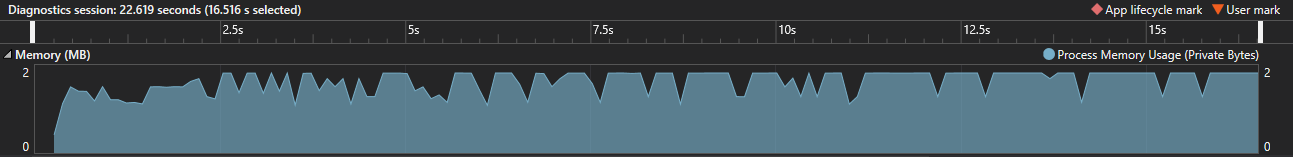
\includegraphics[width=\textwidth]{../figures/poo_mem.png}
\smallskip
\fonte{Autoria própria}
\label{fig:poo_mem}
\end{figure}

O consumo de memória da aplicação com o \textit{Framework} PON C++ 2.0 é
mostrado na Figura \ref{fig:fw2_mem}, é interessante observar a curva crescente
que demonstra que a memória não está sendo corretamente desalocada, fazendo com
que o consumo de memória apenas aumente ao longo do tempo, até o ponto em que a
memória do sistema se esgote e a aplicação falhe. Um teste isolado realizando a
instanciação das entidades uma única vez apresentou um consumo de 69 MB de RAM.
\citeonline{msc_xavier_2014} também já havia encontrado problemas no mecanismo
de alocação de memória do \textit{Framework} PON C++ 2.0, evidenciados neste
experimento.

\begin{figure}[!htb]
\centering
\caption{Consumo de memória \textit{Framework} PON C++ 2.0}
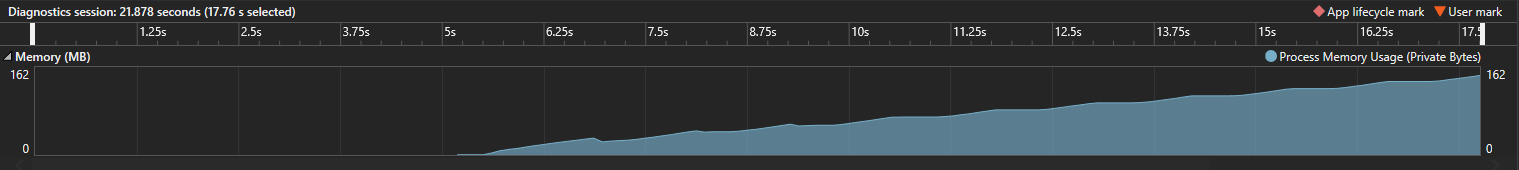
\includegraphics[width=\textwidth]{../figures/fw2_mem.png}
\smallskip
\fonte{Autoria própria}
\label{fig:fw2_mem}
\end{figure}

O consumo de memória da aplicação com o \textit{Framework} PON C++ 4.0 é
mostrado na Figura \ref{fig:fw4_mem}, na qual pode ser observado um
comportamento esperado da memória sendo alocada para as entidades até atingir
cerca de 24 MB, e então sendo apropriadamente desalocada antes da nova iteração,
demonstrando a estabilidade do gerenciamento de memória, sendo realizado com a
utilização dos \textit{smart pointers}.

\begin{figure}[!htb]
\centering
\caption{Consumo de memória \textit{Framework} PON C++ 4.0}
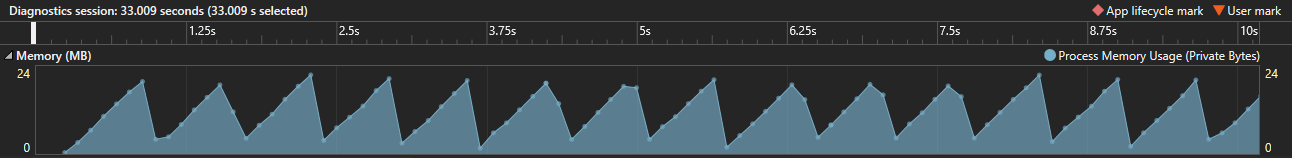
\includegraphics[width=\textwidth]{../figures/fw4_mem.png}
\smallskip
\fonte{Autoria própria}
\label{fig:fw4_mem}
\end{figure}

Desta forma, fica explícito que o \textit{Framework} PON C++ 4.0 apresenta
ganhos de desempenho significativos com relação ao \textit{Framework} PON C++
2.0. No cenário da aplicação de sensores, quando comparado ao \textit{Framework}
PON C++ 2.0, o \textit{Framework} PON C++ 4.0 reduziu em 62\% o tempo de
execução no pior caso, e em 85\% no melhor caso. Além da redução nos tempos de
execução, também reduziu em quase dois terços o consumo de memória e não
apresentou o problema de vazamento de memória apresentado no gráfico da Figura
\ref{fig:fw2_mem}.

Uma aplicação de cunho similar, porém com contexto ainda mais restrito ao grupo
de pesquisa, a aplicação mira ao alvo. Esta aplicação apresenta nível de
complexidade e lógica similares à aplicação de sensores e é apresentada como
curiosidade no \nameref{ap:apendice_mira_alvo}.

\subsection{Aplicação \textit{Bitonic Sort}}\label{sec:bitonic_sort}

O \textit{Bitonic Sort} é um algoritmo de ordenação originalmente proposto por
\citeonline{batcher_68}. Esta seção discorre sobre os detalhes do algoritmo,
assim como sua implementação em PON, apresentando comparações com a
implementação tradicional do algoritmo em linguagem de programação C.

Uma sequência é dita como \textit{bitonic} caso sua primeira parte seja
crescente e a segunda parte decrescente, de forma que para uma sequência \([0
... n-1]\) a mesma é \textit{bitonic} caso exista um índice \textit{i} nos
limites \(0<=i<=n-1\) de modo que \(x_0 <= x_1 <= ... <= x_i\) e \(x_i >=
x_{i+1} >= ... >= x_{n-1}\). Como exemplo, a sequência \([5, 6, 7, 8, 4, 3, 2,
1]\) é \textit{bitonic}, pois pode ser dividida em duas sequências \([5, 6, 7,
8]\) e \([1, 2, 3, 4]\), que são, respectivamente, crescentes e decrescentes.

Desta forma, uma sequência \textit{bitonic} pode ser ordenada por um conjunto de
comparadores que operam em pares de valores da sequência, no contexto da chamada
ordenação \textit{bitonic}. O algoritmo de ordenação \textit{Bitonic Sort} pode
ser dividido em duas etapas, sendo que primeiramente a sequência é transformada
em uma sequência \textit{bitonic} (etapa 1) e subsequentemente essa sequência
\textit{bitonic} é ordenada de forma crescente (etapa 2). Estas duas etapas são
ilustradas na Figura \ref{fig:bitonic_order}. Os comparadores dessas etapas
podem ser executados de forma paralela permitindo melhor desempenho do algoritmo
em ambientes multiprocessados.

\begin{figure}[!htb]
\centering
\caption{Processo de ordenação com \textit{Bitonic Sort}} 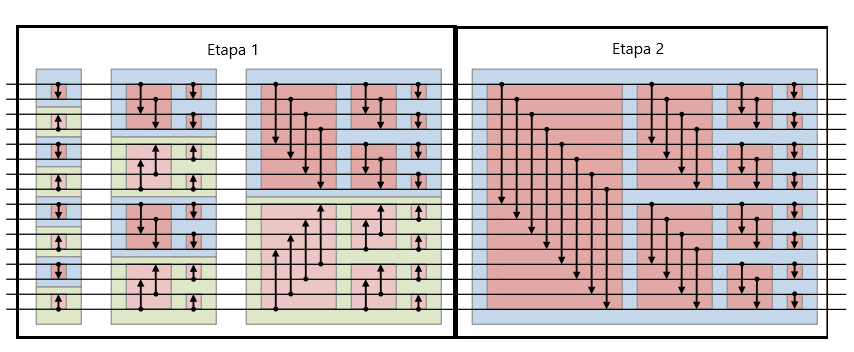
\includegraphics[width=\textwidth]{../figures/bitonic_sort_mod.png}
\smallskip
\caption*{Fonte:
Adaptado de \citeonline{Mullapudi_2014}}
\label{fig:bitonic_order}
\end{figure}

O algoritmo do \textit{Bitonic Sort} pode ser dividido em vários estágios, dado
o fato que as comparações são realizadas entre dois elementos e os mesmos são
comparados apenas uma vez dentro de cada estágio, de tal modo que as comparações
dentro de cada estágio podem ser realizadas de forma paralela. A existência
desses estágios paralelizáveis favorece uma implementação em PON devido ao seu
paralelismo intrínseco. Deste modo, os comparadores do \textit{Bitonic Sort}
podem ser representados por meio de \textit{Rules}
\cite{quali_pordeus_2020,pordeus_2021}.

Em uma interpretação para a implementação em PON os diferentes estágios podem
ser representados por \textit{Attributes} independentes, de modo que a ordenação
ocorre movendo os valores do estágio anterior para o próximo. Assim, cada
comparador é materializado como um \textit{FBE} com duas \textit{Rules},
conforme ilustrado na Figura \ref{fig:rule_bitonic}, sendo que uma \textit{Rule}
opera no caso da comparação ser verdadeira e a outra no caso da comparação ser
falsa. Isto visto que pela divisão em etapas, é necessário mover os valores da
etapa anterior para a próxima, invertendo os valores apenas quando a comparação
é verdadeira. Os métodos \textit{mtMove} e \textit{mtSwap} são responsáveis por
mover os valores de \textit{at1} e \textit{at2} do \textit{FBE} do comparador
atual para os \textit{Attributes} dos comparadores das etapas seguintes.

\begin{figure}[!htb]
\centering
\caption{\textit{Rules} para comparador do \textit{Bitonic Sort} em PON}
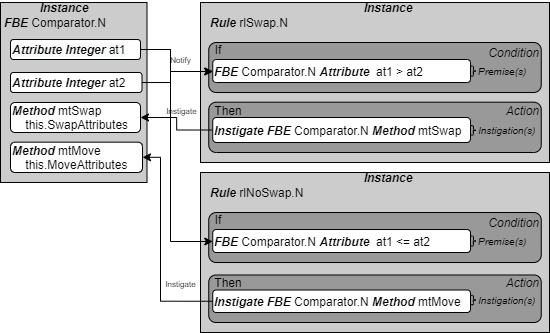
\includegraphics[width=0.9\textwidth]{../figures/rule_bitonic.png}
\smallskip
\fonte{Autoria própria}
\label{fig:rule_bitonic}
\end{figure}

\FloatBarrier

Na estrutura do ordenador implementado com o \textit{Framework} PON C++ 4.0,
todas as entidades do PON são criadas de forma dinâmica na construtora da
\textit{struct}, baseando-se no número de elementos, sendo passado como
parâmetro. A função \textit{Sort}, por sua vez, atribuí os valores aos
\textit{Attributes} pertinentes ao primeiro estágio de comparação, conforme
mostrado no Código \ref{cod:sort_function}, e a ordenação é realizada pela
interação das entidades do PON já declaradas na construção do objeto, ao final
da operação retornando o vetor \textit{out} que armazena os resultados da
ordenação. Devido à extensão dos códigos, essa seção traz apenas trechos das implementações,
com o código completo disponível para referência no \nameref{ap:apendice_bitonic}.

\begin{lstlisting}[caption = {Trecho de código da estrutura NOPBitonicSorter},
  source = {Autoria própria}, float=htb,
  label = {cod:sort_function}]
std::vector<T> NOPBitonicSorter::Sort(const std::vector<T>& input){
    for (auto i = 0; i < input.size(); i++)    {
        elements[1][i]->SetValue(input[i]);
    }
    return out;
}
\end{lstlisting}

Essa implementação apresenta elementos completamente independentes e
paralelizáveis, de modo que qualquer alteração no estado de um
\textit{Attribute} do estágio de entrada do ordenador é refletida na saída do
mesmo. Entretanto, esta implementação em PON apresenta desempenho ruim, devido
ao fato de ser necessário mover os dados entre os diferentes estágios. A
operação de mover os dados necessita da aprovação de uma \textit{Rule} para cada
comparação para sua execução. Além disso, também pode ocorrer execução de
\textit{Rules} desnecessárias decorrentes da ordem de avaliação dos
comparadores, porque os valores nos estágios intermediários são substituídos
pelos estágios anteriores à medida que as \textit{Rules} são aprovadas,
causando a aprovação de regras desnecessárias durante o processo. Dados estes
problemas, se torna necessária uma nova interpretação deste problema em PON por
meio da proposta de uma solução mais eficiente.

Esta solução mais eficiente proposta se aproveita da característica da divisão
em estágios do algoritmo, desta vez não utilizando \textit{Attributes} para os
estágios intermediários, mas sim uma \textit{Premise} adicional aos comparadores
que controla sua execução apenas durante o seu estágio. Desta forma também é
possível reduzir o número de \textit{Rules} pela metade, utilizando apenas uma
\textit{Rule} por comparador. Esta interpretação é representada na Figura
\ref{fig:rule_bitonic_old}.

\begin{figure}[!htb]
\centering
\caption{\textit{Rules} para implementação mais eficiente do comparador do
\textit{Bitonic Sort} em PON}
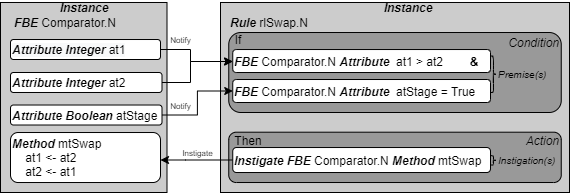
\includegraphics[width=0.95 \textwidth]{../figures/nop_bitonic_old.png}
\smallskip
\fonte{Autoria própria}
\label{fig:rule_bitonic_old}
\end{figure}

O Código \ref{cod:sort_function_stages} mostra em detalhe o corpo da função de
ordenação desta implementação, onde os valores dos \textit{Attributes} são
atribuídos de acordo com o vetor de entrada, porém a ordenação é realizada por
meio da mudança do estado dos \textit{Attributes} de controle de cada estágio
para \textit{true}.

\begin{lstlisting}[caption = {Trecho de código da estrutura NOPBitonicSorterStages},
  source = {Autoria própria}, float=htb,
  label = {cod:sort_function_stages}]
template<typename T>
std::vector<T> NOPBitonicSorterStages::Sort(std::vector<T>& input)
{
    for (size_t i = 0; i < input.size(); i++)
    {
        elements[i]->SetValue(input[i], NOP::NoNotify);
    }
    for (const auto& stage : stages)
    {
        stage->SetValue(true);
        stage->SetValue(false);
    }
    for (auto i = 0; i < elements.size(); i++)
    {
        out[i] = elements[i]->GetValue();
    }
    return out;
}
\end{lstlisting}

\FloatBarrier

A Figura \ref{fig:bitonic_bench_nop} mostra como a implementação com a divisão
em estágios apresenta tempos de execução significativamente menores que a
implementação original em PON, sendo que para o caso da ordenação de 64
elementos a implementação em estágios chega a ser 20.000 vezes mais rápida.

\begin{figure}[!htb]
\centering
\pgfplotstableread{../data/bitonic_nop.data}{\sensorbench}
\begin{tikzpicture}[scale=0.9]
\begin{axis}[width=0.7\linewidth, ylabel=Tempo de execução (ns), ymode=log,
% yticklabel pos=right,
xlabel=Número de elementos, xmin=8, xmax=64, xmode=log, log basis x={2}, legend
pos=north west] \addplot [mark=*, red, thick] table [x={elements}, y={nop}]
{\sensorbench}; \addplot [mark=*, blue, thick] table [x={elements}, y={nop_old}]
{\sensorbench};
\legend{Implementação original, Implementação com estágios}
\end{axis}
\end{tikzpicture}
\caption{Testes de desempenho da aplicação do \textit{Bitonic Sort} com
diferentes implementações em PON}
\fonte{Autoria própria}
\label{fig:bitonic_bench_nop}
\end{figure}

Além disso, o número reduzido de \textit{Rules} utilizadas faz com que a
implementação em estágio tenha o consumo de memória cerca de 50\% menor.
Utilizando as ferramentas de análise do Visual Studio 2019 foi possível traçar o
perfil do consumo de memória das aplicações. Neste teste, para o caso do
ordenador de 1024 elementos, o total de memória alocado pela aplicação chega a
74 MB na implementação original e 35 MB na implementação em estágios. Esse alto
consumo de memória é decorrente do grande número de elementos do PON utilizados
na construção do programa, sendo que para o ordenador de 1024 elementos são
necessários 28.160 comparadores. Os gráficos do consumo de memória para a
implementação original e a implementação em estágios são apresentados nas
Figuras \ref{fig:mem_bitonic} e \ref{fig:mem_bitonic_nop_old} respectivamente.

\begin{figure}[!htb]
\centering
\caption{Consumo de memória para a aplicação do algoritmo \textit{Bitonic Sort}
com o \textit{Framework} PON C++ 4.0 na implementação original}
\smallskip
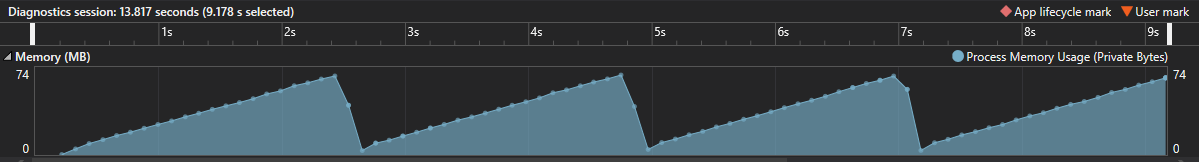
\includegraphics[width=\textwidth]{../figures/mem_bitonic.png}
\fonte{Autoria própria}
\label{fig:mem_bitonic}
\smallskip
\caption{Consumo de memória para a aplicação do algoritmo \textit{Bitonic Sort}
com o \textit{Framework} PON C++ 4.0 na implementação em estágios}
\smallskip
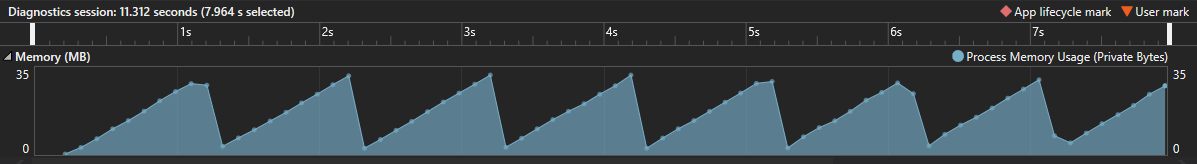
\includegraphics[width=\textwidth]{../figures/mem_bitonic_nop_old.png}
\fonte{Autoria própria}
\label{fig:mem_bitonic_nop_old}
\end{figure}

Além das implementações em PON, foi escolhida uma implementação em C do
algoritmo, disponível na íntegra no \nameref{ap:bitonic_c}\cite{pitsianis_2008}, de modo a
servir como base de comparação para o desempenho da implementação em PON. Nos
testes foi avaliado o tempo de execução para realizar a ordenação de 32, 64,
128, 256, 512, 1024, 2048 e 4096 elementos\footnote{Teste executado em um
computador com processor Ryzen 5 3600 a 3.6GHz e 16 GB de RAM DDR4 a 3000MHz
(dual channel) e sistema operacional Windows 10 64 bits.}. Na avaliação do tempo
de execução da implementação em PON não é considerado o tempo gasto na
inicialização da estrutura em si, mas sim da execução da função \textit{Sort}.
Os resultados são exibidos no gráfico da Figura \ref{fig:bitonic_bench}. Para
esta comparação foi utilizada a implementação em estágios com o PON.

\begin{figure}[!htb]
\centering
\pgfplotstableread{../data/bitonic_bench.data}{\sensorbench}
\begin{tikzpicture}[scale=0.9]
\begin{axis}[width=0.7\linewidth, ylabel=Tempo de execução (ns), ymode=log,
% yticklabel pos=right,
xlabel=Número de elementos, xmin=32, xmax=4096, xmode=log, log basis x={2},
legend pos=north west] \addplot [mark=*, red, thick] table [x={elements},
y={oop}] {\sensorbench}; \addplot [mark=*, blue, thick] table [x={elements},
y={nop}] {\sensorbench}; 
%\addplot [mark=*, green, thick] table [x={elements},y={nop_par}]
%{\sensorbench}; 
\legend{PP em C, \textit{Framework} PON C++ 4.0, \textit{Framework} PON C++ 4.0
paralelizado }
\end{axis}
\end{tikzpicture}
\caption{Testes de desempenho da aplicação do algoritmo \textit{Bitonic Sort}}
\fonte{Autoria própria}
\label{fig:bitonic_bench}
\end{figure}

O tempo de execução do processo de ordenação com o PON foi superior ao da
implementação em C utilizando o PP e, quanto maior o número de elementos, maior a
diferença entre os tempos de execução, chegando a uma diferença de 2000 vezes no
caso de ordenação de 4096 elementos. O problema da implementação em PON se dá
devido ao elevado número de comparadores, que por sua vez representam um número
elevado de entidades do PON instanciadas para a construção do comparador, cada
uma com um significativo custo de memória associado, além do elevado número de
notificações necessárias para a realização do processo de ordenação. 

De forma a aproveitar a natureza paralelizável do algoritmo, também é possível
paralelizar a implementação em PON com o \textit{Framework} PON C++ 4.0, fazendo
usos do mecanismo de notificações paralelas, de forma que cada notificação pode
ser processada em uma \textit{thread} separada, potencialmente reduzindo os
tempos de execução para aplicações com elevado número de entidades a serem
notificadas.

Esta implementação é bastante simples com o \textit{Framework} PON C++ 4.0, pois
basta utilizar a função \textit{SetValue} com um parâmetro de template
\textit{<NOP::Parallel>} para que as notificações sejam realizadas de forma
paralela. O Código \ref{cod:fn_sort_p} mostra a função de ordenação de forma
paralela, similar ao já apresentado no Código \ref{cod:sort_function_stages}.

\begin{lstlisting}[caption = {\textit{Bitonic Sort} paralelizado com o \textit{Framework} PON C++ 4.0},
  source = {Autoria própria}, float=htb,
  label = {cod:fn_sort_p},
]
template<typename T>
std::vector<T> NOPBitonicSorterStages::Sort(std::vector<T>& input)
{
    for (size_t i = 0; i < input.size(); i++)
    {
        elements[i]->SetValue(input[i], NOP::NoNotify);
    }

    for (const auto& stage : stages)
    {
        stage->SetValue<NOP::Parallel>(true);
        stage->SetValue<NOP::Parallel>(false);
    }

    for (auto i = 0; i < elements.size(); i++)
    {
        out[i] = elements[i]->GetValue();
    }

    return out;
}
\end{lstlisting}

No gráfico da Figura \ref{fig:bitonic_par} é possível observar que a
paralelização oferece ganhos de desempenho para a ordenação de números elevados
de elementos, enquanto para números menores de elementos o tempo de execução
aumentou. Por sua vez, na Figura \ref{fig:bitonic_bench_rel}, são comparados os
tempos de execução da aplicação com paralelização relativos aos da execução
sequencial. Para a ordenação de 4096 elementos, a execução de forma
paralelizada teve seu tempo de execução reduzido em cerca de 50\%. 

\begin{figure}[!htb]
\centering
\pgfplotstableread{../data/bitonic_bench.data}{\sensorbench}
\begin{tikzpicture}[scale=0.9]
\begin{axis}[width=0.7\linewidth, ylabel=Tempo de execução (ns), ymode=log,
% yticklabel pos=right,
xlabel=Número de elementos, xmin=32, xmax=4096, xmode=log, log basis x={2},
legend pos=north west] \addplot [mark=*, blue, thick] table [x={elements},
y={nop}] {\sensorbench}; \addplot [mark=*, green, thick] table
[x={elements},y={nop_par}] {\sensorbench}; \legend{\textit{Framework} PON C++
4.0 sequencial, \textit{Framework} PON C++ 4.0 paralelizado}
\end{axis}
\end{tikzpicture}
\caption{Comparação da paralelização na aplicação do algoritmo \textit{Bitonic
Sort}}
\fonte{Autoria própria}
\label{fig:bitonic_par}
\end{figure}

Além de observar os tempos de execução, a fim de verificar os efeitos do
paralelismo nessa aplicação, é possível observar a utilização de CPU durante a
execução, também utilizando as ferramentas de análise do Visual Studio 2019, da
mesma forma que o consumo de memória foi observado nas outras aplicações. 

\begin{figure}[!htb]
  \centering
  \pgfplotstableread{../data/bitonic_bench.data}{\sensorbench}
  \begin{tikzpicture}[scale=0.9]
  \begin{axis}[width=0.7\linewidth, ylabel=Tempo de execução relativo, %ymode=log,
    xlabel=Número de elementos, xmin=32, xmax=4096, xmode=log, log basis x={2},
  legend pos=north west]
  %\addplot[mark=*, green, thick] table[x={elements}, y expr={\thisrow{nop}/\thisrow{oop}}]{\sensorbench};
  \addplot[mark=*, blue, thick] table[x={elements}, y expr={\thisrow{nop_par}/\thisrow{nop}}]{\sensorbench};
  %\legend{\textit{Framework} PON C++ 4.0 sequencial, \textit{Framework} PON C++ 4.0 paralelizado}
  %\horLineFromPoint{1,4096}
  \end{axis}
  \end{tikzpicture}
  \caption{Tempos de execução do algoritmo \textit{Bitonic Sort} com o \textit{Framework} PON C++ 4.0 paralelizado relativo ao sequencial}
  \fonte{Autoria própria}
  \label{fig:bitonic_bench_rel}
  \end{figure}

Ao avaliar o desempenho da aplicação para ordenar 4096 elementos durante a
execução sequencial, com o gráfico da utilização de CPU na Figura
\ref{fig:bit_cpu}, a utilização de CPU não passa de 8\%. Isso se dá pelo fato do
ambiente de testes possuir 12 núcleos, de modo que uma aplicação sem paralelismo
executando de forma sequencial somente consegue utilizar um dos núcleos,
equivalente a 8.33\% do processamento disponível.

\begin{figure}[!htb]
\centering
\caption{Utilização de CPU durante execução do algoritmo \textit{Bitonic Sort}
com o \textit{Framework} PON C++ 4.0 sequencial}
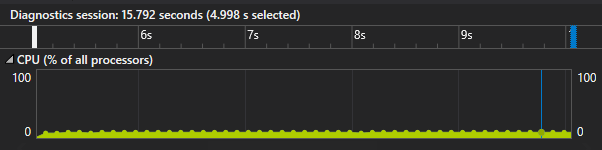
\includegraphics[width=\textwidth]{../figures/cpu_bitonic.png}
\smallskip
\fonte{Autoria própria}
\label{fig:bit_cpu}
\end{figure}

Já a implementação paralelizada consegue fazer uma utilização muito melhor da
CPU. Como ilustrado na \ref{fig:bit_cpu_par}, a utilização de CPU varia,
atingindo quase 100\% em alguns momentos. Ou seja, essa implementação utiliza de
melhor forma os recursos disponíveis, com isso atingindo um desempenho melhor
que a implementação sequencial.

\begin{figure}[!htb]
\centering
\caption{Utilização de CPU durante execução do algoritmo \textit{Bitonic Sort}
com o \textit{Framework} PON C++ 4.0 paralelizado}
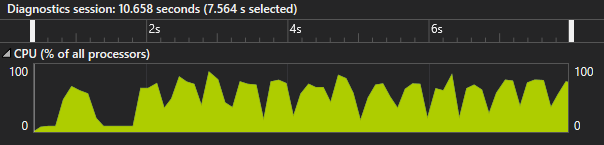
\includegraphics[width=\textwidth]{../figures/cpu_bitonic_par.png}
\smallskip
\fonte{Autoria própria}
\label{fig:bit_cpu_par}
\end{figure}

\subsection{Aplicação \textit{Random Forest}}\label{sec:random_forest}

O \textit{Random Forest} é um algoritmo popular de aprendizado de máquina,
utilizado em muitas aplicações para classificação e regressão. O algoritmo
consiste em um conjunto de árvores de decisão, treinadas individualmente e
combinadas para obter um resultado com menor erro de classificação/regressão.
Para esta aplicação é comparado o desempenho da implementação em PON com
implementações em linguagem de programação \textit{Python} e C. Em tempo, Python
é linguisticamente mais alto-nível que a linguagem C justamente.

Isto dito, no \textit{Random Forest}, cada árvore é avaliada separadamente,
viabilizando a execução de maneira paralela. Ao final da execução de todas as
árvores os resultados são combinados para todo o conjunto \cite{criminisi_2011}.
A Figura \ref{fig:random_forest} ilustra a estrutura das árvores de decisão
(\textit{decision trees}) independentes do \textit{Random Forest}. No contexto
do PON, a implementação do \textit{Random Forest} é interessante devido ao fato
deste algoritmo ser construído essencialmente por meio de expressões lógicas
\textit{if-else}. Deste modo, o PON pode permitir eliminar as redundâncias
temporais e estruturais, além de também permitir a paralelização da execução das
árvores \cite{quali_pordeus_2020}.

\begin{figure}[!htb]
  \centering
  \caption{Árvores de decisão do algoritmo \textit{Random Forest}}
  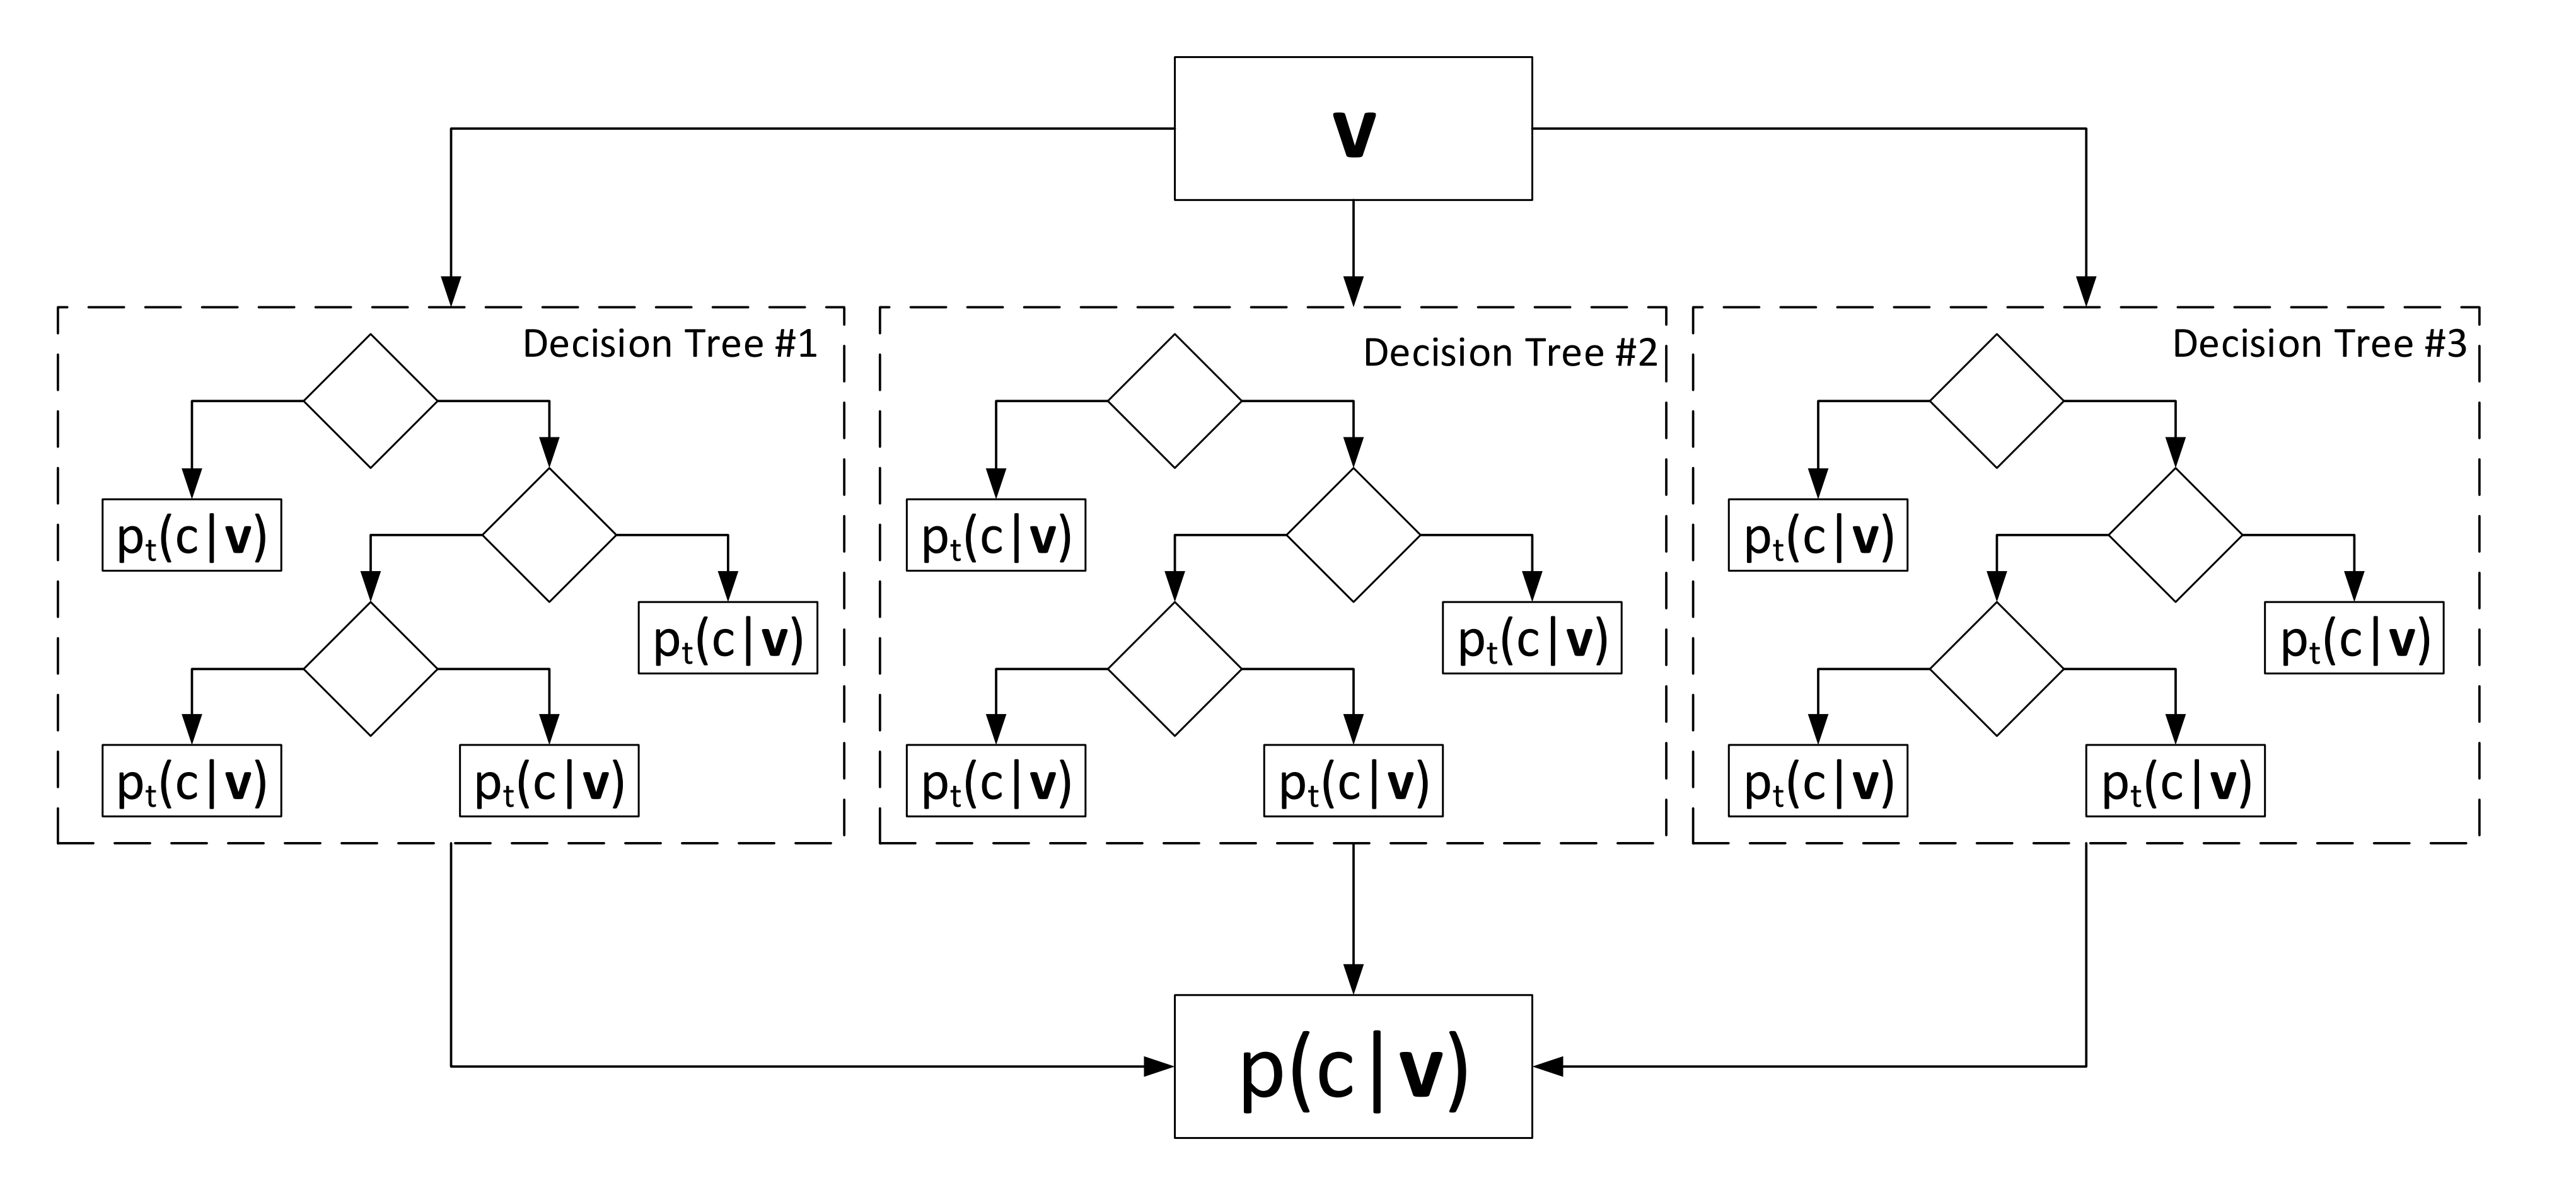
\includegraphics[width=0.7\textwidth]{../figures/random_forest.png}
  \smallskip
  \fonte{\citeonline{quali_pordeus_2020}}
  \label{fig:random_forest}
  \end{figure}

Uma implementação realizada originalmente por \citeonline{quali_pordeus_2020}
\footnote{Implementação disponível em
\url{https://github.com/leonardopordeus/RP}} possibilita a geração de código em
PON com base nas árvores de decisão geradas com o auxílio da biblioteca
scikit-learn\footnote{Maiores detalhes sobre a biblioteca podem ser encontrados
em \url{https://scikit-learn.org/stable/}} na linguagem de programação Python.
Esta implementação era capaz de gerar código específico para o PON em LingPON e
PON-HD, assim como para o PP em linguagem de programação C. Esta implementação
foi modificada para gerar código específico para o PON utilizando o
\textit{Framework} PON C++ 4.0, com base na implementação para geração de código
em LingPON já existente. A implementação em proposta neste trabalho contempla
apenas a utilização do algoritmo para a classificação de dados, sendo que o
treinamento e geração das árvores de classificação são realizados por meio do
uso da biblioteca scikit-learn.

No Código \ref{cod:rule_rf} é apresentado como
exemplo uma das \textit{Rules} geradas por esta implementação. Esta
\textit{Rule} é composta por diversas \textit{Premises} que são capazes de
avaliar o valor de \textit{Attributes}, que representam os dados de entrada da
classificação, com relação aos valores atribuídos durante o processo de
treinamento das árvores. Ainda, devido a extensão dos códigos gerados aqui são
disponibilizados apenas trechos, com o código-fonte completo para o caso de uma
árvore disponível no \nameref{ap:rf}.

\begin{lstlisting}[caption = {\textit{Rule} do algoritmo \textit{Random Forest} para o \textit{Framework} PON C++ 4.0},
  source = {Autoria própria}, %float=htb,
  label = {cod:rule_rf},
]
/*
rule rlTree_0_5
      premise prTree_0_5_1
        this.attr3 > 75
      end_premise
      and
      premise prTree_0_5_2
        this.attr2 <= 495
      end_premise
      and
      premise prTree_0_5_3
        this.attr3 <= 165
      end_premise
      and
      premise prTriggerTree0
        this.trigger_tree_0 == true
      end_premise
  end_condition
  action sequential
      instigation sequential
        call this.mt_count_versicolor()
        call this.mtTrigger1()
        call this.mtRstTrigger0()
      end_instigation
  end_action
end_rule
*/
NOP::SharedRule rlTree_0_5 = NOP::BuildRule(
        NOP::BuildCondition<NOP::Conjunction>(
            NOP::BuildPremise(attr3, 75, NOP::Greater()),
            NOP::BuildPremise(attr2, 495, NOP::LessEqual()),
            NOP::BuildPremise(attr3, 165, NOP::LessEqual()),
            NOP::BuildPremise(trigger_tree_0, true, NOP::Equal())
        ),
        NOP::BuildAction(
            NOP::BuildInstigation(mt_count_versicolor,mtTrigger1,mtRstTrigger0)
       )
    );
\end{lstlisting}

O algoritmo \textit{Random Forest} possibilita a utilização de um número
variável de árvores de decisão. Dessa forma, com a implementação supracitada,
também é possível gerar código para diferentes números de árvores. Nos testes
foram utilizados os valores de 1, 10, 20, 50 e 100 árvores. Na Tabela
\ref{tab:elementos_arvores} são relacionados os números de elementos necessários
para a construção de cada versão do classificador com diferentes números de
árvores.

\begin{table}[!htb]
\centering
\label{tab:elementos_arvores}
\smallskip
\begin{tabularx}{0.8\textwidth}{|c|X|X|X|X|X|}
\hline
\textbf{Número de árvores} & 1 & 10 & 20 & 50 & 100\\
\hline
\hline
\textit{Attributes} & 7 & 34 & 64 & 154 & 304 \\
\hline
\textit{Premises} & 8 & 39 & 56 & 80 & 93 \\
\hline
\textit{Conditions} & 9 & 90 & 173 & 437 & 839 \\
\hline
\textit{Rules} & 9 & 90 & 173 & 437 & 839 \\
\hline
\textit{Actions} & 6 & 60 & 120 & 300 & 600 \\
\hline
\textit{Instigations} & 6 & 60 & 120 & 300 & 600 \\
\hline
\textit{Methods} & 6 & 60 & 120 & 300 & 600 \\
\hline
\end{tabularx}
\caption{Número de elementos em relação ao número de árvores}
\fonte{Autoria própria}
\end{table}

Esse elevado número de entidades e, por sua vez, de linhas de código faz com que
o tempo de compilação dessa aplicação seja bastante elevado. No computador
utilizado nos testes, com processor Ryzen 5 3600 e 16 GB de RAM DDR4, o tempo de
compilação da aplicação de testes chegou a ser superior a 3 minutos, pois
somente o arquivo contendo o código-fonte definindo a estrutura das árvores
contém mais de 32.000 linhas de código.

A Figura \ref{fig:rf_bench} exibe o resultado dos testes de tempo de execução
das diferentes implementações do algoritmo \textit{Random Forest}. As
implementações em PP (C) e PON (C++) utilizam o código gerado, enquanto a
aplicação em linguagem de programação Python utiliza a função disponível na
própria biblioteca, \textit{model.predict(data)}. O desempenho deste algoritmo
em PON, com o uso do \textit{Framework} PON C++ 4.0, foi muito inferior ao
desempenho da implementação em linguagem de programação C. Ainda assim, os
tempos de execução foram menores que os da aplicação em linguagem de programação
Python.

\begin{figure}[!htb]
  \centering
  \pgfplotstableread{../data/random_forest.data}{\sensorbench}
  \begin{tikzpicture}[scale=0.9]
  \begin{axis}[width=0.7\linewidth, ylabel=Tempo de execução (ns), ymode=log,
  % yticklabel pos=right,
  xlabel=Número de árvores, xmin=1, xmax=100, xmode=log, legend pos=north west]
  \addplot [mark=*, red, thick] table [x={n}, y={vivado}] {\sensorbench};
  \addplot [mark=*, blue, thick] table [x={n}, y={nop}] {\sensorbench}; \addplot
  [mark=*, green, thick] table [x={n},y={py}] {\sensorbench}; \legend{PP em C,
  \textit{Framework} PON C++ 4.0, Python}
  \end{axis}
  \end{tikzpicture}
  \caption{Testes de desempenho da aplicação do algoritmo \textit{Random
  Forest}}
  \fonte{Autoria própria}
  \label{fig:rf_bench}
  \end{figure}

Além disso, ao contrário da aplicação \textit{Bitonic Sort}, a aplicação de
paralelismo, usando a função \textit{SetValue<NOP::Parallel>}, não resultou em
redução nos tempos de execução. Conforme pode ser observado na Figura
\ref{fig:random_forest_par} a implementação paralelizada aumentou os tempos de
execução quando comparada com a implementação sequencial. Isso pode ser
justificado pelo fato da implementação utilizar diversos \textit{Attributes} e
\textit{Premises} de gatilho, que, na prática, forçam a execução de certas
etapas a ocorrer de forma sequencial, limitando os benefícios da paralelização.
Ainda, conforme o gráfico da Figura \ref{fig:random_forest_rel} que ilustra o
tempo de execução da implementação paralelizada relativo ao da implementação
sequencial, a implementação paralelizada apresenta tempos de execução pelo menos
cinco vezes mais lentos.

\begin{figure}[!htb]
\centering
\pgfplotstableread{../data/random_forest.data}{\sensorbench}
\begin{tikzpicture}[scale=0.85]
\begin{axis}[width=0.7\linewidth, ylabel=Tempo de execução (ns), ymode=log,
% yticklabel pos=right,
xlabel=Número de árvores, xmin=1, xmax=100, xmode=log, legend pos=north west]
\addplot [mark=*, blue, thick] table [x={n}, y={nop}] {\sensorbench}; \addplot
[mark=*, green, thick] table [x={n},y={nop_par}] {\sensorbench};
\legend{\textit{Framework} PON C++ 4.0 sequencial, \textit{Framework} PON C++
4.0 paralelizado}
\end{axis}
\end{tikzpicture}
\caption{Comparação da paralelização na aplicação do algoritmo \textit{Random
Forest}}
\fonte{Autoria própria}
\label{fig:random_forest_par}
\end{figure}

\begin{figure}[!htb]
\centering
\pgfplotstableread{../data/random_forest.data}{\sensorbench}
\begin{tikzpicture}[scale=0.85]
\begin{axis}[width=0.7\linewidth, ylabel=Tempo de execução relativo, %ymode=log,
  % yticklabel pos=right,
  xlabel=Número de árvores, xmin=1, xmax=100, xmode=log, legend pos=north west]
%\addplot[mark=*, green, thick] table[x={elements}, y expr={\thisrow{nop}/\thisrow{oop}}]{\sensorbench};
\addplot[mark=*, blue, thick] table[x={n}, y expr={\thisrow{nop_par}/\thisrow{nop}}]{\sensorbench};
%\legend{\textit{Framework} PON C++ 4.0 sequencial, \textit{Framework} PON C++ 4.0 paralelizado}
%\horLineFromPoint{1,4096}
\end{axis}
\end{tikzpicture}
\caption{Tempos de execução do algoritmo \textit{Random
Forest} com o \textit{Framework} PON C++ 4.0 paralelizado relativo ao sequencial}
\fonte{Autoria própria}
\label{fig:random_forest_rel}
\end{figure}

Para avaliar a utilização de CPU foi utilizada a implementação do algoritmo
utilizando 100 árvores. Do mesmo modo que a aplicação \textit{Bitonic Sort}, a
utilização de CPU para a implementação sequencial do \textit{Random Forest}
também fica limitada a 8\%. Diferente do observado na aplicação \textit{Bitonic
Sort}, a utilização de CPU para a implementação sequencial do \textit{Random
Forest} não utiliza de forma eficiente todos os núcleos da CPU. De acordo com a
Figura \ref{fig:rf_cpu_par}, o consumo de CPU fica próximo de apenas 50\%. Isto
é refletido no resultado dos tempos de execução que não apresentam redução na
execução paralelizada.

Em suma, foi concluído que nesta implementação do algoritmo \textit{Random
Forest} em \textit{Framework} PON C++ 4.0, a utilização de \textit{Attributes} e
\textit{Premises} de gatilho limitam a paralelização. Essa limitação na
paralelização faz com que não seja possível utilizar de forma equilibrada todos
os núcleos da CPU, de modo que o desempenho não apresenta benefícios com a
execução paralelizada. De fato, ocorre justamente o contrário, pois o custo de
execução dos mecanismos de paralelização sobrepassa os benefícios de desempenho
da  mesma, aumentando o tempo de execução total da aplicação.

\begin{figure}[!htb]
\centering
\caption{Utilização de CPU durante execução do algoritmo \textit{Random Forest}
com o \textit{Framework} PON C++ 4.0 sequencial}
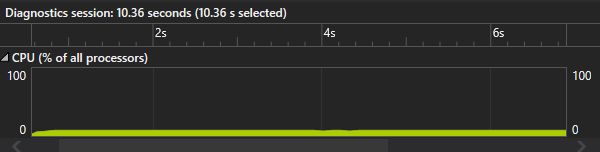
\includegraphics[width=\textwidth]{../figures/cpu_rf.png}
\smallskip
\fonte{Autoria própria}
\label{fig:rf_cpu}
\end{figure}

\begin{figure}[!htb]
\centering
\caption{Utilização de CPU durante execução do algoritmo \textit{Random Forest}
com o \textit{Framework} PON C++ 4.0 paralelizado}
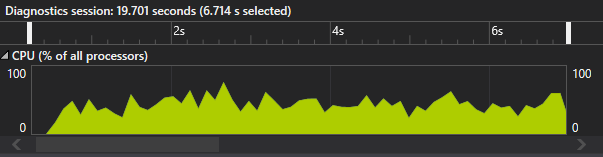
\includegraphics[width=\textwidth]{../figures/cpu_rf_par.png}
\smallskip
\fonte{Autoria própria}
\label{fig:rf_cpu_par}
\end{figure}


\subsection{Aplicação de Controle de Tráfego Automatizado (CTA)}\label{sec:semaforo}

A aplicação de Controle de Tráfego Automatizado (CTA) é mais um caso de estudo frequentemente
utilizado para avaliar o desempenho do PON. Esta aplicação foi escolhida por
permitir avaliar o \textit{Framework} PON C++ 4.0  do ponto de vista de
implementação do paralelismo, por meio da comparação com outro
\textit{framework} que materializa esta propriedade, o \textit{Framework} PON
Elixir/Erlang \cite{msc_negrini_2019}.

O ambiente de simulação desta aplicação proposto por \citeonline{renaux_2015} é
composto por uma matriz 10x10, com um total de 100 interseções. As linhas e
colunas da matriz representam ruas enquanto as interseções representam os
cruzamentos com semáforos. Uma representação gráfica deste ambiente é
apresentada na Figura \ref{fig:cta_renaux}.

\begin{figure}[!htb]
\centering
\caption{Ambiente de simulação}
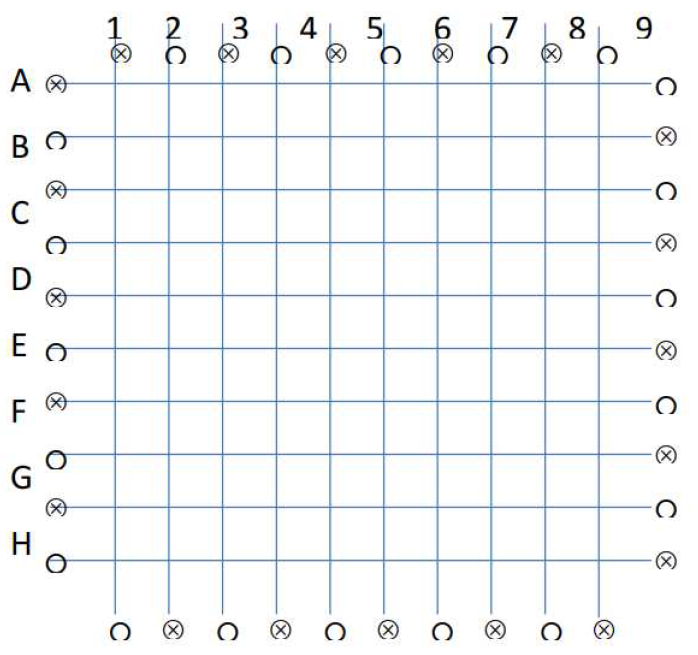
\includegraphics[width=0.72\textwidth]{../figures/semaforos_renaux.png}
\smallskip
\fonte{\citeonline{renaux_2015}}
\label{fig:cta_renaux}
\end{figure}

Neste experimento são consideradas duas estratégias que regem o comportamento
dos semáforos, a estratégia de controle independente e estratégia de controle
baseado em congestionamento facilitado (CBCF). Na estratégia de controle
independente cada semáforo possui tempos fixos para cada estado
\cite{msc_negrini_2019}. O diagrama de estados com a temporização para esta
estratégia é apresentado na Figura \ref{fig:estados_cta}. Neste diagrama as
cores representam o estado em si (verde, amarelo e vermelho), enquanto os
círculos H representam o estado do semáforo da via horizontal do cruzamento, e o
círculo V representa o estado  do semáforo da via vertical, de acordo com a
disposição apresentada na Figura \ref{fig:cta_renaux}.

\begin{figure}[!htb]
\centering
\caption{Estados do CTA com estratégia independente}
\smallskip
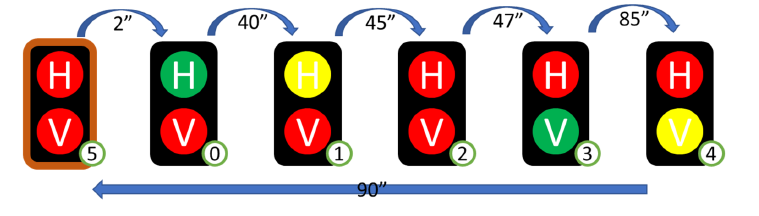
\includegraphics[width=0.75\textwidth]{../figures/estados_cta.png}
\fonte{\citeonline{msc_negrini_2019}}
\label{fig:estados_cta}
\end{figure}

\FloatBarrier

Na estratégia de controle CBCF, diferente da estratégia independente, um sensor
é utilizado para detectar a porcentagem de veículos parados, sendo que se o
sensor detecta que a porcentagem de veículos parados está acima de 60\% e o
tempo total do semáforo vermelho é menor que 30 segundos, ele tem seu tempo
ajustado para 30 segundos. O diagrama de estados para esta estratégia é
ilustrado na Figura \ref{fig:estados_cbcf}.

\begin{figure}[!htb]
\centering
\caption{Estados do CTA com estratégia CBCF}
\smallskip
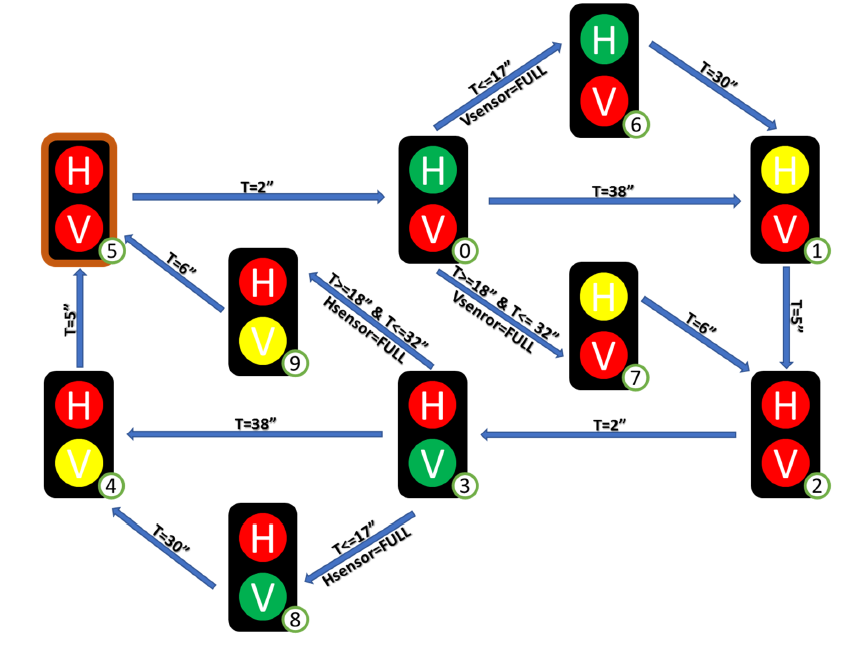
\includegraphics[width=0.85\textwidth]{../figures/estados_cbcf.png}
\fonte{\citeonline{msc_negrini_2019}}
\label{fig:estados_cbcf}
\end{figure}

Para a execução deste experimento, foi utilizado código em LingPON tanto para a
aplicação o \textit{Framework} PON C++ 4.0 como para o \textit{Framework} PON
Elixir/Erlang. Devido às limitações atuais no compilador LingPON para
\textit{Framework} PON C++ 4.0, o código foi modificado apenas de forma a
utilizar o mecanismo de notificações paralelas (com
\textit{SetValue<NOP::Parallel>}). O Código \ref{cod:semaforo} apresenta um
trecho deste código em LingPON, enquanto o Código \ref{cod:semaforo_fw}
apresenta um trecho do código gerado em \textit{Framework} PON C++ 4.0, contendo
um \textit{Method} e uma \textit{Rule}, para o \textit{FBE} do semáforo na
estratégia independente. Os códigos-fonte completos são disponibilizados no
\nameref{ap:cta}.

\begin{lstlisting}[caption = {Trecho do FBE para o CTA na estratégia independente em LingPON},
  source = {Autoria própria}, float=htb, language=nopl,
  label = {cod:semaforo},
]
fbe Semaphore_CTA
    private integer atSemaphoreState = 5
    public integer atSeconds = 0
    private method mtResetTimer
        assignment
            this.atSeconds = 0
        end_assignment
    end_method
    private method mtHorizontalTrafficLightGREEN
        assignment
            this.atSemaphoreState = 0
        end_assignment
    end_method    
    ...
    rule rlHorizontalTrafficLightGreen
        condition
                premise prSeconds
                    this.atSeconds == 2
                end_premise
                and
                premise prSemaphoreState
                    this.atSemaphoreState == 5
                end_premise
        end_condition
        action sequential
            instigation parallel
                call this.mtHorizontalTrafficLightGREEN()
            end_instigation
        end_action
    end_rule
    ...
end_fbe
\end{lstlisting}

\begin{lstlisting}[caption = {Trecho do FBE para o CTA na estratégia independente em \textit{Framework} PON C++ 4.0},
  source = {Autoria própria}, float=htb,
  label = {cod:semaforo_fw},
]
SemaphoreCTA::SemaphoreCTA()
    : atSeconds{NOP::BuildAttribute<int>(0)},
      atSemaphoreState{NOP::BuildAttribute<int>(5)},
      prSeconds{NOP::BuildPremise<>(atSeconds, 2, NOP::Equal())},
      prSemaphoreState{
          NOP::BuildPremise<int>(atSemaphoreState, 5, NOP::Equal())},
      ...
    rlHorizontalTrafficLightGreen = NOP::BuildRule(
        NOP::BuildCondition(CONDITION(*prSeconds && *prSemaphoreState),
                            prSeconds, prSemaphoreState),
        NOP::BuildAction(NOP::BuildInstigation<NOP::Parallel>(
            METHOD(mtHorizontalTrafficLightGREEN();)))

    );
    ...
}

void SemaphoreCTA::mtHorizontalTrafficLightGREEN()
{
    atSemaphoreState->SetValue<NOP::Parallel>(0);
}
\end{lstlisting}

\FloatBarrier

O experimento utilizado para a avaliação de desempenho consiste em iterar quatro
mil vezes em uma matriz 10x10 de semáforos, sendo que cada iteração incrementa o
tempo do \textit{Attribute} \textit{atSeconds} de cada semáforo. Desta forma, o
experimento permite avaliar o tempo de execução da lógica, sem considerar o
tempo de espera real entre os estados do semáforo, que existiriam em uma
situação prática, mas que não são relevantes do ponto de vista de desempenho.

Para fins de comparação com o \textit{Framework} PON Elixir/Erlang são
considerados os resultados apresentados por \citeonline{msc_negrini_2019}
utilizando o ambiente VM16, que utiliza uma instância de ambiente virtualizado
na nuvem da Amazon com processadores AMD EPYC série 7000 com 16 núcleos a uma
frequência de \textit{clock} de 2,5 GHz em todos os núcleos
\cite{msc_negrini_2019}, enquanto os experimentos com o \textit{Framework} PON
C++ 4.0 \textit{Framework} utilizaram um processador Ryzen 5 3600 com 6 núcleos
e 12 \textit{threads} a 3,6 GHz.

\FloatBarrier

O consumo de memória da aplicação durante a execução com a estratégia de
controle independente atingiu um máximo de 2,7 MB, enquanto para a estratégia de
controle CBCF o consumo de memória checou a 4,8 MB, devido ao maior número de
\textit{Rules} utilizadas neste método de controle. O consumo de memória durante
a execução das duas estratégias é mostrado nas Figuras \ref{fig:mem_cta} e
\ref{fig:mem_cbcf}. A aplicação com o \textit{Framework} PON Elixir/Erlang
consumiu, respectivamente, cerca de 800 MB e 700 MB nas estratégias independente
e CBCF.

\begin{figure}[!htb]
\centering
\caption{Consumo de memória para a aplicação de semáforo com estratégia
independente com o \textit{Framework} PON C++ 4.0}
\smallskip
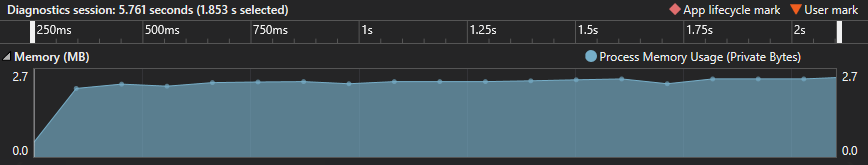
\includegraphics[width=\textwidth]{../figures/cta_mem.png}
\fonte{Autoria própria}
\label{fig:mem_cta}
\end{figure}

\begin{figure}[!htb]
\centering
\caption{Consumo de memória para a aplicação de semáforo com estratégia CBCF com
o \textit{Framework} PON C++ 4.0}
\smallskip
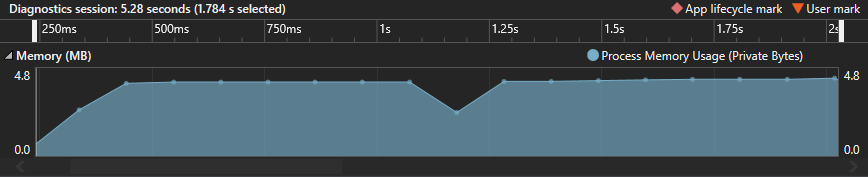
\includegraphics[width=\textwidth]{../figures/cbcl_mem.png}
\fonte{Autoria própria}
\label{fig:mem_cbcf}
\end{figure}

De modo a observar a paralelização o uso de CPU também foi observado o uso de
CPU durante a execução das duas estratégias. Como pode ser observado nos
gráficos das Figuras \ref{fig:cpu_cta} e \ref{fig:cpu_cbcf}, o uso de CPU oscila
entre cerca de 40\% e 70\% em ambos os cenários.

\begin{figure}[!htb]
\centering
\caption{Uso de CPU durante execução do Semáforo com estratégia independente com
o \textit{Framework} PON C++ 4.0}
\smallskip
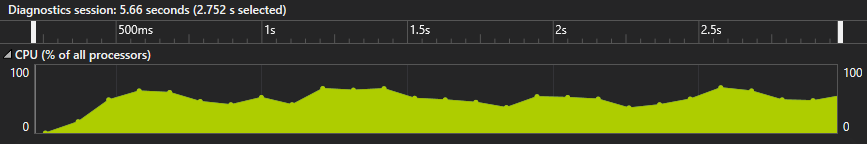
\includegraphics[width=\textwidth]{../figures/cta_cpu.png}
\fonte{Autoria própria}
\label{fig:cpu_cta}
\end{figure}

\begin{figure}[!htb]
\centering
\caption{Uso de CPU durante execução de semáforo com estratégia CBCF com o
\textit{Framework} PON C++ 4.0}
\smallskip
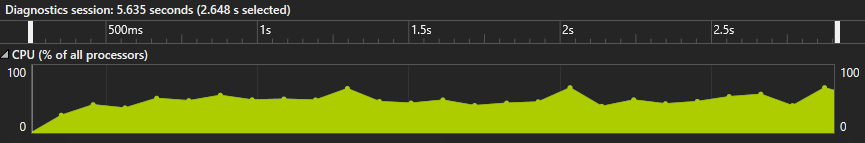
\includegraphics[width=\textwidth]{../figures/cbcl_cpu.png}
\fonte{Autoria própria}
\label{fig:cpu_cbcf}
\end{figure}
\FloatBarrier

O tempo de execução das estratégias de controle independente e CTBF foram de 336
ms e 434 ms respectivamente, utilizando o \textit{Framework} PON C++ 4.0. No
caso dos testes com o \textit{Framework} PON Elixir/Erlang os tempos de execução
foram de 4.703 ms e 8.525 ms. Esses resultados são comparados no gráfico da
Figura \ref{fig:fw4_elixir}. A aplicação com o \textit{Framework} PON C++ 4.0
apresenta tempos de execução uma ordem de grandeza inferiores aos tempos de
execução da mesma aplicação com o \textit{Framework} PON Elixir/Erlang, mesmo
considerando a execução da aplicação em Elixir/Erlang em um ambiente com poder
de processamento muito superior, além de apresentar consumo de memória mais de
cem vezes menor.

\begin{figure}[!htb]
\centering
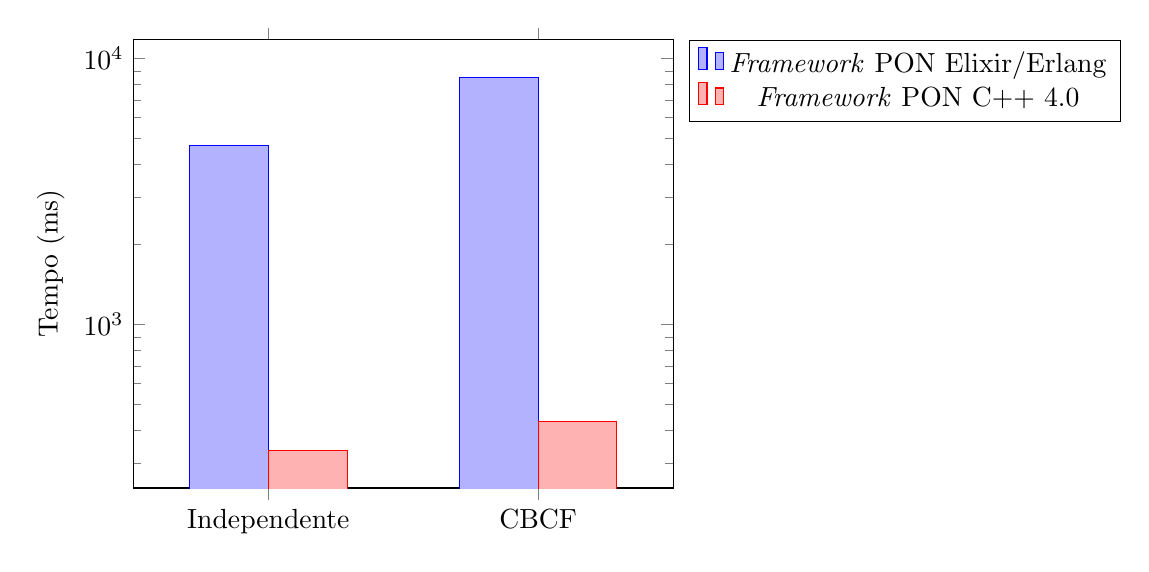
\begin{tikzpicture}
  \begin{axis}[ybar=0pt,
    %ymin=0,
    samples=2, domain=1:2, xtick=data, bar width=1cm, enlarge x
    limits={abs=0.5}, legend pos=outer north east, ylabel={Tempo (ms)},
    xticklabels={Independente, CBCF}, ymode = log ]
  \addplot 
    coordinates {(0,4703) (1,8525)};
  \addplot 
    coordinates {(0,336) (1,434)}; \legend{\textit{Framework} PON
  Elixir/Erlang,\textit{Framework} PON C++ 4.0}
  \end{axis}
  \end{tikzpicture}
\caption{Tempo de execução da aplicação de semáforo com o \textit{Framework}
PON C++ 4.0 \textit{Framework} PON Elixir/Erlang}
\fonte{Autoria própria}
\label{fig:fw4_elixir}
\end{figure}
%estrategia fw4       elixir ind        335937500 4703000000 cbcf
%433593750 8525000000

O desempenho superior do \textit{Framework} PON C++ 4.0 era esperado, visto que
Elixir é uma linguagem de programação de mais alto nível, utilizando o PF, com
maior grau de abstração, que por sua vez é associada a custos computacionais
elevados quando comparado a uma linguagem como C++. O objetivo desta comparação
não é apenas observar como aplicações em C++ possuem desempenho superior a
aplicações com Elixir/Erlang, pois ambas as linguagens de programação têm
propostas diferentes, mas sim demonstrar no contexto do PON como o
\textit{Framework} PON C++ 4.0 permite o desenvolvimento de aplicações que usam
paralelismo ao mesmo tempo que consegue entregar um alto desempenho com baixos
tempos de execução e baixo consumo de memória, o que não é possível com outros
\textit{frameworks} do PON.

\section{Jogo NOPUnreal com \textit{Framework} PON C++
4.0}\label{sec:nopunreal4}

O jogo apresentado na Seção \ref{sec:nopunreal}, desenvolvido com o
\textit{Framework} PON C++ 2.0, foi reimplementado com o \textit{Framework} PON
C++ 4.0 de forma a permitir comparar a verbosidade do código nas duas
implementações. A implementação é feita em parte diretamente no POO, utilizando
as bibliotecas da Unreal Engine principalmente para os cálculos matemáticos e
implementações de nível gráfico da \textit{engine} em si, enquanto a parte do
jogo relativa ao PON é dada pela lógica de controle automatizado dos inimigos.
No total, o jogo contém 17 \textit{Rules} em sua composição.

A implementação com o \textit{Framework} PON C++ 4.0 utiliza
como base a implementação original com o \textit{Framework} PON C++ 2.0,
utilizando a mesma estrutura de classes, apenas modificando o código referente
às \textit{Rules}. Desta forma o diagrama de classes, apresentado na Figura
\ref{fig:jogo_fw4}, é equivalente ao da Figura \ref{fig:jogo_fw2}. 
Como ambos os \textit{frameworks} apresentam funcionalidades equivalentes o
processo de implementação com o \textit{Framework} PON C++ 4.0 foi bastante
simples, bastando converter o formato de código das estruturas do PON para o
modelo do novo \textit{framework}. Esse processo levou apenas uma tarde de
trabalho. Como resultado, as funcionalidades do jogo foram mantidas.

\begin{figure}[!htb]
\centering
\caption{Diagrama de classes do jogo desenvolvido com o \textit{Framework} PON
C++ 4.0 }
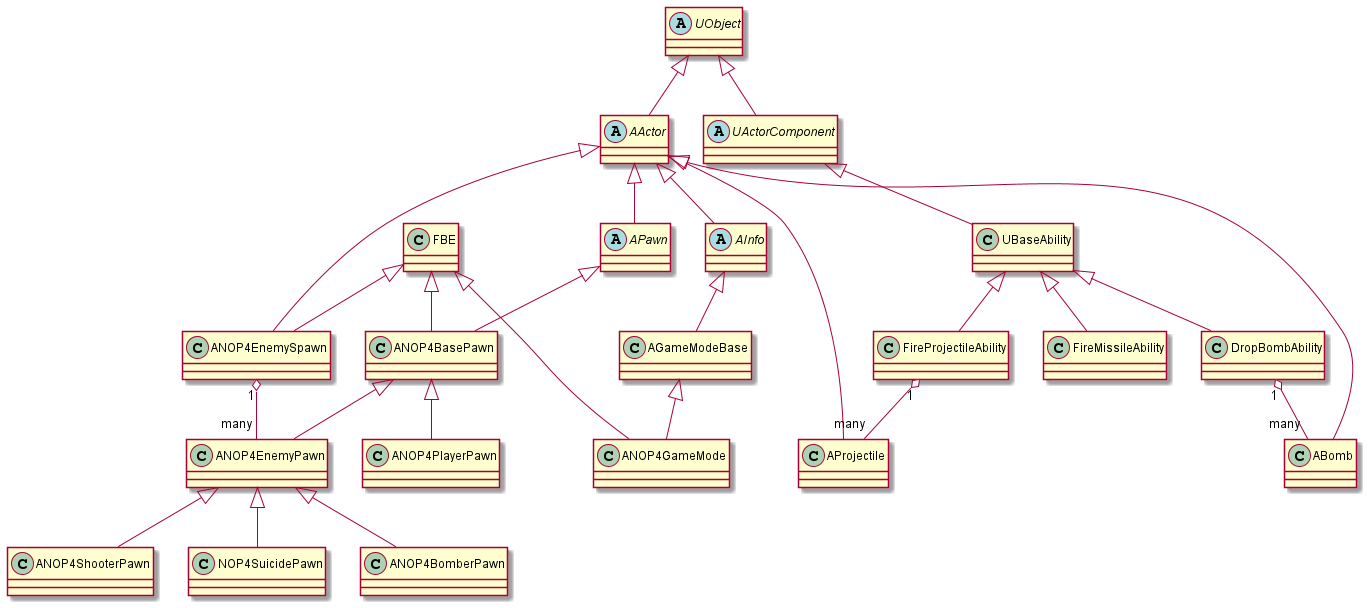
\includegraphics[width=\textwidth]{../out/diagrams/class_diagram_nop4/NOP4Unreal.png}
\smallskip
\fonte{Autoria própria}
\label{fig:jogo_fw4}
\end{figure}

Foi comparada a diferença na quantidade de código necessária para implementar o
jogo utilizando o POO em C++, o \textit{Framework} PON C++ 2.0 e o
\textit{Framework} PON C++ 4.0. Utilizando a ferramenta
\textit{cloc}\footnote{Ferramenta disponível em
\url{https://github.com/AlDanial/cloc}}, foi avaliado o número de linhas
contidas nos códigos que compõem cada uma destas implementações. Conforme
apresentado na Tabela \ref{tab:linhas_de_codigo_nopunreal}, a implementação com
o \textit{Framework} PON C++ 4.0 conseguiu reduzir em 14.75\% o número de linhas
de código quando comparado com a implementação com o \textit{Framework} PON C++
2.0, e possui apenas 7.6\% mais linhas de código que a implementação com o POO
em C++. A implementação com o \textit{Framework} PON C++ 4.0 permitiu converter
diretamente o código com o \textit{Framework} PON C++ 2.0 ao mesmo tempo que
simplificou o código reduzindo o número de linhas de código totais.

\begin{table}[!htb]
\centering
\caption{Linhas de código para a composição do jogo NOPUnreal}
\smallskip
\begin{tabularx}{0.8\textwidth}{|X|X|}
\hline
Versão & Linhas de código\\
\hline
POO em C++ & 1407 \\
\hline
\textit{Framework} PON C++ 2.0 & 1776 \\
\hline
\textit{Framework} PON C++ 4.0 & 1514 \\
\hline
\end{tabularx}
\fonte{Autoria própria}
\label{tab:linhas_de_codigo_nopunreal}
\end{table}

\section{Pesquisa de opinião de desenvolvedores}\label{sec:opiniao}

De forma a permitir avaliar os resultados referentes à facilidade de uso de
\textit{framework}, que é algo que não há como avaliar de forma objetiva, apenas
subjetiva, foi montado um questionário com diversas questões referentes ao uso
dos \textit{frameworks} do PON. O questionário completo está disponível no
\nameref{ap:questionario}. O resultado desta pesquisa é apresentado meramente a
fim de curiosidade, por contar com uma amostra muito pequena sem significância
estatística devido ao pequeno número de desenvolvedores que já utilizaram o
\textit{Framework} PON C++ 4.0. O questionário contou com apenas três
respostas\footnote{Respostas dos alunos do grupo de pesquisa do PON Lucas Skora,
Gustavo Chierici e Lucas Mamann.}, sendo que todas estas três pessoas possuem
experiência utilizando tanto o \textit{Framework} PON C++ 4.0 como o
\textit{Framework} PON C++ 2.0.

Foi perguntado aos desenvolvedores, numa escala de 0 a 5, o quanto consideravam
que o \textit{Framework} PON C++ 4.0 apresenta melhorias sobre o
\textit{Framework} PON C++ 2.0. Como pode ser observado na Figura
\ref{fig:fw_compare}, é consenso entre os desenvolvedores que o
\textit{Framework} PON C++ 4.0 apresenta melhorias significativas sobre o
\textit{Framework} PON C++ 2.0.

\begin{figure}[!htb]
\centering
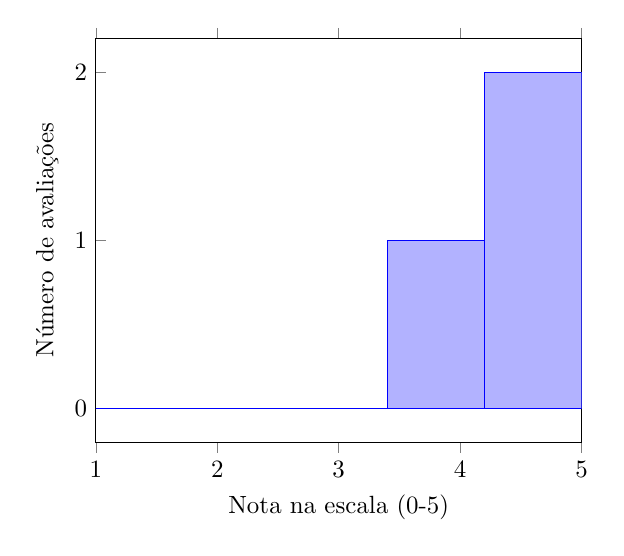
\begin{tikzpicture}[scale=0.9]
\begin{axis}[xmin=1, xmax=5, ybar, ytick = {0,1,2}, xlabel=Nota na escala (0-5),
ylabel=Número de avaliações] \addplot+[hist={bins=5}] table[row sep=\\,y
index=0] {data\\
  4\\ 5\\ 5\\
};
\end{axis}
\end{tikzpicture}
\caption{Resultado da pesquisa de avaliação da melhoria do \textit{Framework}
PON C++ 4.0 sobre o \textit{Framework} PON C++ 2.0}
\fonte{Autoria própria}
\label{fig:fw_compare}
\end{figure}

Em maiores detalhes, foi requisitado aos desenvolvedores avaliar ambos os
\textit{frameworks} de acordo com diversos critérios, como facilidade de
aprendizado, facilidade de uso, verbosidade, versatilidade, desempenho e
aderência aos fundamentos do PON. Para cada critério o usuário pode responder
com fraco, moderado, satisfatório, muito bom ou excelente. Para facilitar a
visualização dos resultados as respostas foram convertidas para uma escala de 1
a 5, onde 1 representa fraco, e 5 excelente, e o resultado considera a média
aritmética das respostas. Conforme apresentado no gráfico da Figura
\ref{fig:fw_compare2}, o \textit{Framework} PON C++ 4.0 é considerado  superior
em todos os critérios avaliados.

\begin{figure}[!htb]
\centering
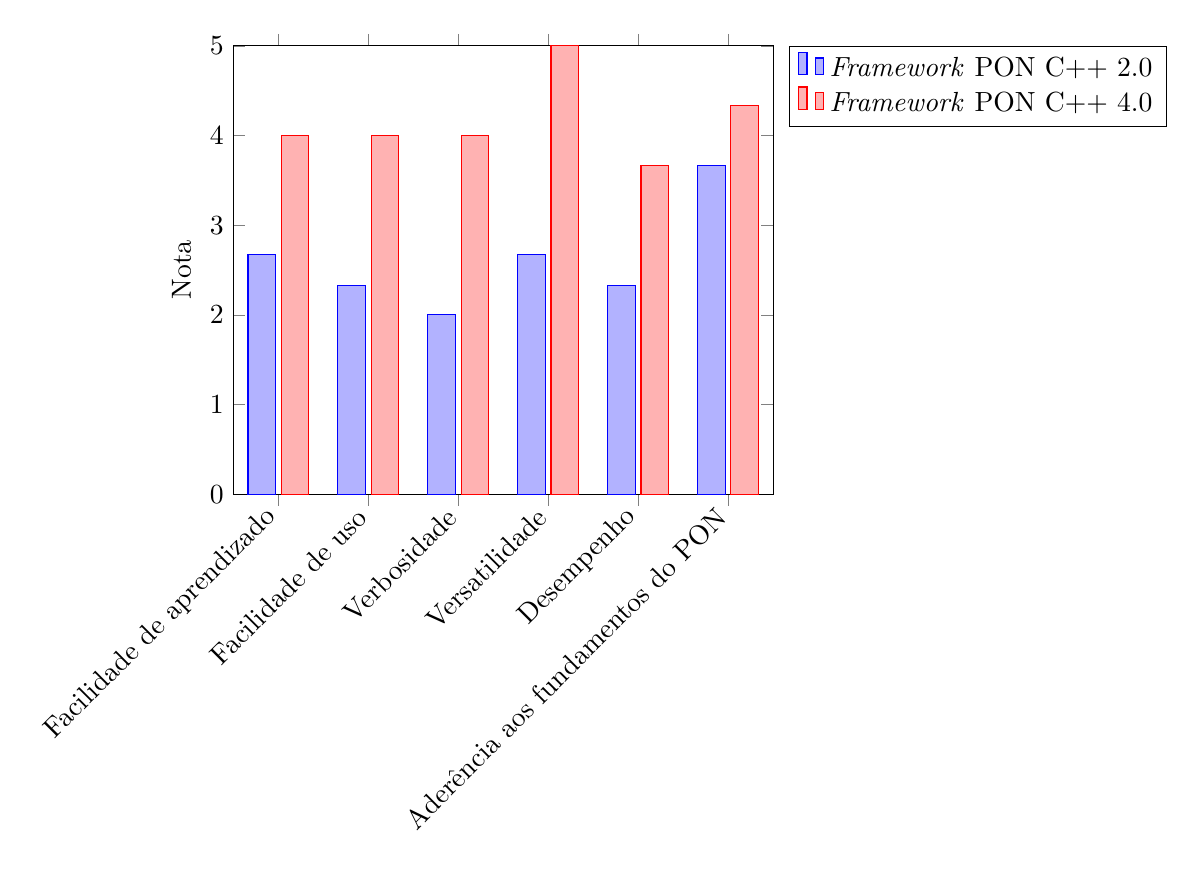
\begin{tikzpicture}
  \begin{axis}[ymin = 0, ymax = 5,%ytick = {0,1,2,3,4,5},
    legend pos=outer north east,
    %x tick label style={      /pgf/number format/1000 sep=},
    ylabel=Nota,
    %enlargelimits=0.05, legend style={at={(0.5,-0.1)}, anchor=north,legend
    %columns=-1},
    ybar,% interval=0.7,
    xticklabels={dummy, Facilidade de aprendizado, Facilidade de uso,
    Verbosidade, Versatilidade, Desempenho, Aderência aos fundamentos do PON}, x
    tick label style={rotate=45,anchor=east}]
  \addplot 
    coordinates {(0,2.67) (1,2.33) (2,2) (3,2.67) (4,2.33) (5,3.67)};
  \addplot 
    coordinates {(0,4) (1,4) (2,4) (3,5) (4,3.67) (5,4.33)};
        \legend{\textit{Framework} PON C++ 2.0,\textit{Framework} PON C++ 4.0}
  \end{axis}
  \end{tikzpicture}
\caption{Resultado da pesquisa de avaliação da melhoria do \textit{Framework}
PON C++ 4.0 sobre o \textit{Framework} PON C++ 2.0}
\fonte{Autoria própria}
\label{fig:fw_compare2}
\end{figure}

\section{Reflexões sobre os resultados obtidos}\label{sec:fw4_reflex}

Por meio dos testes unitários realizados, é possível afirmar que o
\textit{Framework} PON C++ 4.0 consegue atender de forma satisfatória as
funcionalidades necessárias para a construção de aplicações em PON. Considerando
as implementações atuais, é possível comparar a diferença na quantidade de
código necessária para implementar o \textit{Framework} PON C++ 2.0 e o
\textit{Framework} PON C++ 4.0. Utilizando a ferramenta \textit{cloc}, foi
avaliado o número de linhas contidas nos códigos que compõem o
\textit{Framework} PON C++ 2.0 e o \textit{Framework} PON C++ 4.0. Nessa
comparação são consideradas apenas as linhas de código, desconsiderando linhas
em branco e comentários.

\begin{table}[!htb]
\centering
\caption{Linhas de código para a composição do \textit{framework}}
\smallskip
\begin{tabularx}{0.8\textwidth}{|X|X|}
\hline
Versão & Linhas de código\\
\hline
\textit{Framework} PON C++ 2.0 & 6587 \\
\hline
\textit{Framework} PON C++ 4.0 & 970 \\
\hline
\end{tabularx}
\fonte{Autoria própria}
\label{tab:linhas_de_codigo}
\end{table}

A grande diferença no número de linhas de código se dá principalmente pela
estrutura genérica do \textit{Framework} PON C++ 4.0 que permite eliminar a
repetição de código que era presente no \textit{Framework} PON C++ 2.0. Essa
redução no número de linhas de código é importante, pois isso facilita a
manutenção do código por outros desenvolvedores, pois reduz o tamanho da base de
código com a qual um novo desenvolvedor precisa se habituar ao trabalhar com o
código, assim como torna mais simples eventuais alterações e melhorias na
estrutura do \textit{framework}.

Dentre os objetivos da implementação do \textit{Framework} PON C++ 4.0 estão
aumentar facilidade de uso e reduzir da curva de aprendizado, entretanto esses
critérios são bastante subjetivos. Ademais, com o desenvolvimento do jogo
NOPUnreal foi possível constatar de forma objetiva a simplificação do código por
meio da redução do número de linhas de código utilizadas na implementação do
mesmo com o \textit{Framework} PON C++ 4.0 quando comparado com a implementação
com o \textit{Framework} PON C++ 2.0.

A adição de novos recursos da linguagem de programação C++ ao \textit{Framework}
PON C++ 4.0, como o uso de \textit{smart pointers}, e o uso de expressões
\textit{lambda}, além de facilitar o uso e desenvolvimento, não trouxe prejuízos
no desempenho uma vez comparado com o \textit{Framework} PON C++ 2.0 quando
aplicado para o desenvolvimento da aplicação de sensores, sendo que o
\textit{Framework} PON C++ 4.0 apresentou tempos de execução menores que o
\textit{Framework} PON C++ 2.0 neste caso. Entretanto, essa melhoria de
desempenho ainda não foi suficiente a ponto de superar o desempenho da aplicação
no POO em C++ para este cenário.

No entanto, a utilização desses recursos mais avançados do C++ no
\textit{Framework} PON C++ 4.0 causa um aumento na complexidade do código,
principalmente quando comparado com o \textit{Framework} PON C++ 2.0, devido à
utilização de construções mais novas e com sintaxe rebuscada (como expressões
\textit{lambdas}, \textit{fold expressions}). Ainda assim são apresentadas
soluções que permitem abstrair essas construções mais complexas de modo
suficiente para facilitar a aplicação por desenvolvedores com conhecimento menos
avançado dessas sintaxes.

O desenvolvimento da aplicação \textit{Bitonic Sort} demonstra o potencial do
PON para o desenvolvimento de algoritmos paralelizáveis, apesar dos elevados
tempos de execução e consumo de memória, visto que parte destes custos
computacionais podem ser atribuídos à implementação do \textit{Framework} PON
C++ 4.0.

Além disso, ao se avaliar o desempenho da versão paralelizada da aplicação
\textit{Bitonic Sort} pode se observar que a aplicação da paralelização no
mecanismo de notificações pode resultar em ganhos de desempenho referentes ao
tempo de execução em determinados cenários. Porém, a paralelização também pode
causar degradação no desempenho, como no caso da aplicação \textit{Random
Forest}, dependendo da estrutura da aplicação, devido ao natural custo
computacional atrelado ao processo de execução de \textit{threads} em C++.

Nem toda aplicação que pode ser paralelizada consegue obter ganhos de
desempenho como, por exemplo, a implementação do algoritmo \textit{reverse} da
STL paralelizado, que no compilador para C++ da Microsoft (MSVC) teve desempenho
1.6 vezes mais lento que a implementação sequencial. Isso não significa que
estes algoritmos não devam ser paralelizados, mas sim que o \textit{hardware}
atual para o qual o código é compilado não traz ganho de desempenho
\cite{oneal_2018}.

Por fim, principalmente durante o desenvolvimento das aplicações para os
algoritmos \textit{Bitonic Sort} e \textit{Random Forest}, foi possível
constatar a maneira como o \textit{Framework} PON C++ 4.0 facilita o
desenvolvimento de aplicações em PON, pois o desenvolvimento destas mesmas
aplicações com o \textit{Framework} PON C++ 2.0 não foi realizado justamente por
ser extremamente complicada. Por exemplo, na implementação do algoritmo para o
\textit{Bitonic Sort}, as \textit{Rules} são criadas de forma dinâmica durante a
inicialização, o que só foi possível realizar de forma simples devido aos
facilitadores de desenvolvimento, por meio dos \textit{Builder} e gerenciamento
de memória com \textit{smart pointers}, introduzidos pelo \textit{Framework} PON
C++ 4.0.

O \textit{Framework} PON C++ 4.0 avança sobre o que já havia sido apresentado no
\textit{Framework} PON C++ 2.0 no que diz respeito à programação em alto nível
ao disponibilizar interfaces de programação mais fáceis de utilizar, dessa forma
contribuindo para a programação em alto nível. O \textit{Framework} PON C++ 4.0
também é o primeiro \textit{framework} na linguagem C++ a contemplar de forma
satisfatória a propriedade de paralelismo do PON, ao usar recursos
modernos da linguagem C++ que permitem o desenvolvimento de aplicações
\textit{multithread} de forma bastante simples. Os benefícios da aplicação do
paralelismo no \textit{framework} são particularmente destacados nos resultados
da aplicação \textit{Bitonic Sort} apresentados na Seção \ref{sec:bitonic_sort},
enquanto na Seção \ref{sec:random_forest}, com a aplicação do algoritmo
\textit{Random Forest}, demonstra que existem casos em que a paralelização pode
não trazer melhorias ao desempenho. Em suma, os benefícios da paralelização
dependem das características da aplicação, sendo que o \textit{Framework} PON
C++ 4.0 disponibiliza as ferramentas necessárias que permitem ao desenvolvedor
facilmente utilizar a paralelização.

Além disso, no tocante à propriedade do paralelismo, o desenvolvimento da
aplicação de controle de semáforos permitiu comparar o \textit{Framework} PON
C++ 4.0 com o \textit{Framework} PON Elixir/Erlang. Com este experimento, fica
demonstrada a capacidade de paralelismo do \textit{Framework} PON C++ 4.0, cujos
níveis de utilização de CPU atingiram níveis altos, comparáveis aos do
\textit{Framework} PON Elixir/Erlang, ao mesmo tempo que mantém tempos de
execução mais baixos, característicos das implementações de \textit{framework}
do PON em C++. O \textit{Framework} PON C++ 4.0 consegue materializar
propriedades de desempenho e paralelismo do PON simultaneamente, algo que não
foi atingido por nenhum dos outros \textit{frameworks} existentes.

No que diz respeito ao desempenho, como era esperado, o \textit{Framework} PON
C++ 4.0 não consegue apresentar os ganhos esperados quando comparado a
aplicações no PI devido ao alto custo computacional das estruturas utilizadas na
composição do \textit{framework} em si. Entretanto, quando comparado com as
outras materializações em C++, é possível constatar que o \textit{Framework} PON
C++ 4.0 apresenta uma melhora no desempenho das aplicações, reduzindo tanto os
tempos de execução como consumo de memória.

%Deste modo o \textit{Framework} PON C++ 4.0 introduz o conceito de
%\textit{Condition} flexível, definido como a capacidade de se criar
%\textit{Conditions} baseadas em expressões \textit{booleanas} entre
%\textit{Premises}. Esse conceito foi explorado em detalhe na Seção
%\ref{sec:condition}.